\documentclass[%
11pt,%
%oneside,%
twoside,%
%twocolumn,%
titlepage,%
%fleqn,%
%a4page,%
german,%
headsepline%
]{scrartcl}

%\usepackage{fancyhdr}
%\usepackage{scrpage2}
\usepackage{lastpage}
\usepackage{geometry}
\usepackage{graphicx}
\usepackage[utf8]{inputenc}
\usepackage[ngerman]{babel}
\usepackage{lscape}
\usepackage{mymath}
\usepackage{units}
\usepackage{nicefrac}
%\usepackage{pgf,tikz}
\usepackage{pgf,tikz,pgfplots}
\pgfplotsset{compat=1.14}
\usepackage{mathrsfs}
\usetikzlibrary{arrows}
\usepackage{colortbl}
\usepackage{hhline}
\usepackage{multirow}
\usepackage[extendedchars]{grffile}
\usepackage{caption}
\usepackage{multicol,calc}
\usepackage{blindtext}
\usepackage{pdfpages}
\usepackage{hyperref}
\usepackage{tikz-er2}
\usepackage{framed}
\usetikzlibrary{arrows}
\usetikzlibrary{positioning}
\usetikzlibrary{shadows}
\usepackage{rotating}
\usepackage{xr}
\usepackage{pifont}
\usepackage[scanall]{psfrag} % Strings in Bildern durch LaTeX-Texte ersetzen
\usepackage[xspace]{ellipsis} % bessere \dots
%\usepackage{picins}
\usepackage{calc} % rechnen
\usepackage{lscape} % Querformat
\usepackage{longtable} % mehrseitige Tabellen
\usepackage{tabulary} % Tabellen mit automatischer Spaltenberechnung
\usepackage[defblank]{paralist} % erweiterte Listen


%\usepackage{romannum}
\usepackage{longtable}
\usepackage{listings}
\usepackage{wrapfig}
\usepackage{pst-plot}
\usepackage{pstricks}
\usepackage{pstricks-add}
\usepackage[symbol]{footmisc}
\usepackage{xr}
\usepackage[ngerman]{varioref}

\newcommand{\ufrac}[2]{\ensuremath{\,\frac{\mathrm{#1}}{\mathrm{#2}}}}
\newcommand{\name}[1]{\textsc{#1}}

\newcommand{\zitat}[1]{\flqq #1\frqq}
\newcommand{\rede}[1]{``#1''}
\newcommand{\begriff}[1]{``#1''}
\newcommand{\quasi}[1]{``#1''}
\newcommand{\begriffinrede}[1]{`#1'}

\newcommand{\result}[1]{\underline{\underline{#1}}}

\clubpenalty=10000 \widowpenalty=10000


% Command, um Tabellen-Spalten anzupassen
\newcommand{\spaltenheight}{\rule{0mm}{3ex}}
\newcommand{\spaltenwidth}{\rule{3cm}{0mm}}
\newcommand{\spaltensep}{\\[1ex]}
%\arrayrulecolor{darkgreen}
\doublerulesepcolor{white}
\definecolor{lightyellow}{rgb}{1,1,0.8}
\definecolor{Gray}{gray}{0.9}

\newenvironment{system}{\begin{displaymath}
  \left| 
    \begin{array}{rcl}}{\end{array} \right| 
\end{displaymath}}

\newlength{\psein}


% Pagestyle/Layout
%\geometry{a4paper , tmargin =2.5cm,	bmargin=3cm, lmargin =2.5cm,	rmargin =2.5cm,	headheight=3em, headsep=1em, footskip=1cm}
\setlength{\parindent}{0pt} \setlength{\parskip}{1em}
%f\"ur TwoSide
%\lehead{\headmark\pagemark}
%\cehead{}
%\rehead{}
%\lohead{}
%\cohead{}
%\rohead{\headmark}
%f\"ur OneSide
%\ihead{}
%\chead{}
%\ohead{}
%\setheadsepline{0.5pt} % Linie zur Begrenzung
%\setfootsepline{0.5pt} % Linie zur Begrenzung
\pagestyle{headings} % gemachte Einstellungen anwenden


\subject{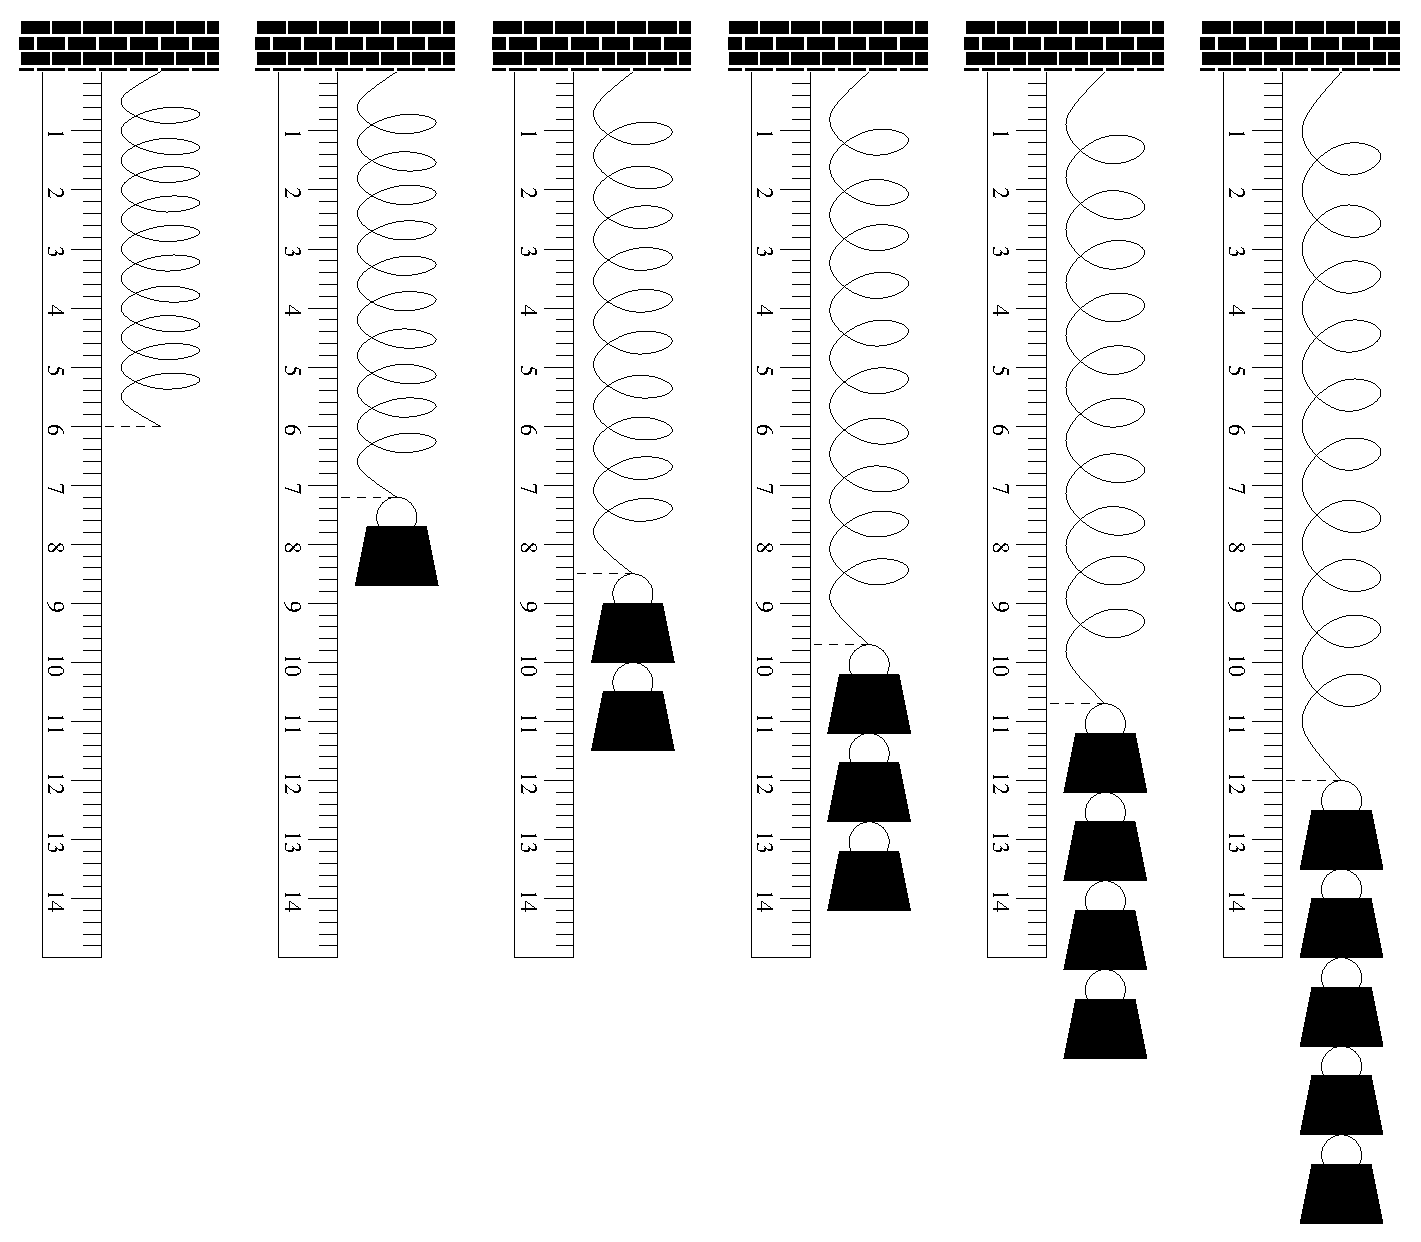
\includegraphics[width=0.618\textwidth]{pictures/feder.eps}}
\title{Lineare Funktionen}
\subtitle{Was heisst linear?}
\author{}
\date{}
%\lowertitleback{
%\includegraphics[height=1.1cm]{/Users/jormawassmer/Pictures/logokoeniz.jpg}%
%\copyright Jorma Wassmer
%1. Auflage, Februar 2011
%}


\begin{document}
\maketitle
\tableofcontents
%\thispagestyle{empty}
\cleardoublepage
%\setcounter{page}{1}

In Wissenschaft und Technik werden oft Zusammenh\"ange zwischen Gr\"ossen betrachtet. Solche Zusammenh\"ange werden durch sogenannte Funktionen mathematisch beschrieben. Funktionen lassen sich mittels Tabellen, Graphiken und Gleichungen beschreiben. In diesem Kapitel besch\"aftigen wir uns mit linearen Funktionen, die graphisch durch Geraden beschrieben werden. Dabei lernen wir den Begriff der Proportionalit\"at besser kennen.

\section{Fallendes H\"utchen}
\label{linfkt1:bsp}

Wir lassen ein Papierh\"utchen fallen und fragen uns: Wie f\"allt das H\"utchen? Wird es immer schneller oder f\"allt es mit konstanter (d.h. gleich bleibender) Geschwindigkeit? Wie k\"onnen wir die Bewegung m\"oglichst vollst\"andig erfassen?

Die Idee ist die Folgende: Die Bewegung besteht ja darin, dass das H\"utchen zu jedem Zeitpunkt an einem bestimmten Ort (d.h. auf einer bestimmten H\"ohe) ist. Deshalb bestimmen wir zu jedem Zeitpunkt den seit dem Start zur\"uckgelegten Weg des H\"utchens. Nat\"urlich k\"onnen wir nicht wirklich zu \emph{jedem} Zeitpunkt den Ort des H\"utchens bestimmen. Deshalb tun wir es z.B. nach jeder vollen Sekunde. 

Das wird uns eine brauchbare Beschreibung der Bewegung liefern, aus der wir Schl\"usse ziehen k\"onnen: Falls z.B. die Streckenabschnitte immer gr\"osser werden, wird das H\"utchen immer schneller. Bleiben sie gleich, f\"allt es mit konstanter Geschwindigkeit.

Die Zeitintervalle (Sekunden) gibt ein Metronom vor. Die (seit dem Start) zur\"uckgelegte Strecke messen wir mit einem Metermass.

\begin{table}[b!]
  \centering
  \begin{tabular}{|c|c|}
    \hline
    t\,[s] & s\,[m] \\ \hline\hline
	0 & 0 \\ \hline
	1 & 0.86 \\ \hline
	2 & 1.53 \\ \hline
	3 & 2.34 \\ \hline
	4 & 3.22 \\ \hline
	5 & 3.89 \\ \hline
	6 & 4.73 \\ \hline
  \end{tabular}
  \caption{Fallendes Papierh\"utchen: $t$: Zeit, $s$: Strecke --- In eckigen Klammern sind die Einheiten angegeben.}
  \label{tab:linfkt1:hut}
\end{table}

Wenn wir die Bewegung des H\"utchens \"uber eine bestimmte Zeit beschreiben wollen, m\"ussen wir viele Messungen durchf\"uhren. Diese k\"onnen wir in einer Tabelle zusammenfassen: siehe \ref{tab:linfkt1:hut}. Jede Tabellenzeile besteht aus einem $t$-$s$-Paar, wobei $t$ f\"ur die Zeit steht und $s$ f\"ur die Strecke. Die dritte Zeile besteht z.B. aus dem Paar $t=2$ und $s=1.53$, wobei wir die Einheiten (Sekunde und Meter) weggelassen haben. Jedes solche Paar k\"onnen wir in einer Kurzschreibweise zusammenfassen: z.B. $(t|s)=(2|1.53)$. 

Die Messungen k\"onnen wir graphisch darstellen, indem wir jedes $(t|s)$-Paar als Punkt in ein Koordinatensystem einzeichnen: siehe \ref{fig:linfkt1:sthut}.



\begin{figure}[b!]
\centering
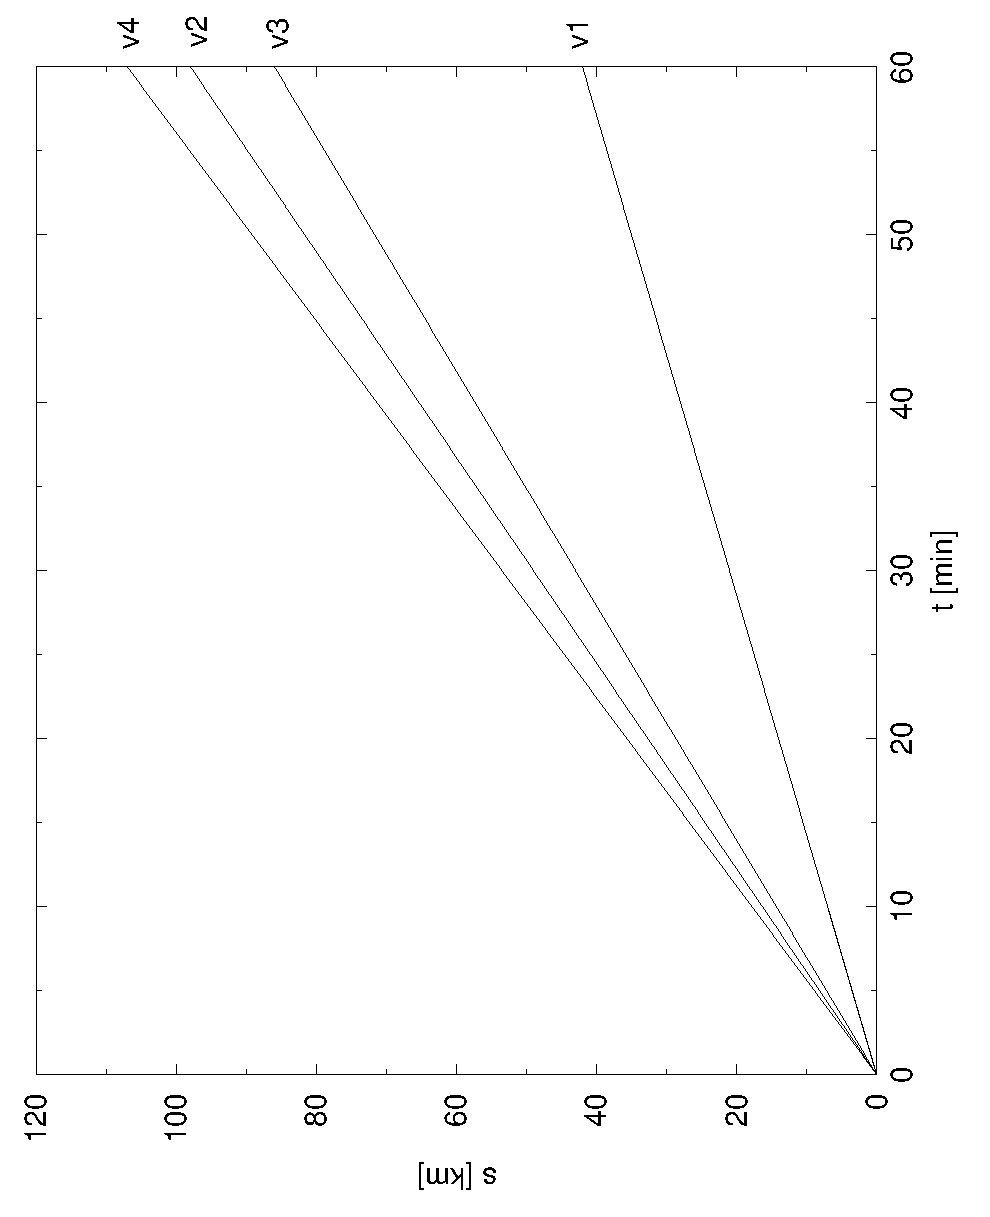
\includegraphics[width=\columnwidth]{pictures/vierzug.eps}
\caption{Weg-Zeit-Diagramm (kurz: $s$-$t$-Diagramm) des H\"utchens: Die Messpunkte werden durch die eingezeichnete Gerade angen\"ahert. Wie \"ublich ist die Zeit waagrecht aufgetragen.}
\label{fig:linfkt1:sthut}
\end{figure}

\section{Was ist eine Funktion?}
\label{linfkt1:was}

In der Tabelle haben wir jedem Zeitpunkt eine Strecke zugeordnet. Dasselbe geschieht in der Graphik: Zu jedem Zeitpunkt ist die zugeh\"orige Strecke als Punkt eingetragen. Eine solche Zuordnung von einer Gr\"osse zur anderen nennen wir \emph{Funktion}.

\begin{quotation}
  Eine Funktion ist eine Zuordnung von einer Gr\"osse zur anderen: Jedem Wert der einen Gr\"osse wird ein Wert der anderen zugeordnet. Eine Funktion k\"onnen wir durch eine Tabelle darstellen oder durch eine Graphik.  
\end{quotation}

Die zur\"uckgelegte Strecke h\"angt von der Zeit ab. Die Funktion gibt an, \emph{wie} die Strecke von der Zeit abh\"angt, d.h. sie beschreibt die Abh\"angigkeit der Strecke von der Zeit. Man sagt: Die Strecke ist \emph{als Funktion der Zeit} dargestellt (d.h. \rede{in Abh\"angigkeit von der Zeit}).

Es kommt immer wieder vor, dass eine Gr\"osse in Abh\"angigkeit (oder eben als Funktion) einer anderen Gr\"osse dargestellt wird. Weitere Beispiele:
\begin{itemize}
\item An eine Spiralfeder werden Metallst\"ucke angeh\"angt. Die Verl\"angerung der Feder h\"angt von der angeh\"angten Masse ab, d.h. letztlich von der Gewichtskraft. Anders formuliert: die Verl\"angerung ist eine Funktion der Kraft.
\item \ref{fig:linfkt1:temp} zeigt den Temperaturverlauf innerhalb eines Tages, wie er an einem bestimmten Ort gemessen wurde. Jedem Zeitpunkt ist eine bestimmte Temperatur zugeordnet, d.h. die Temperatur ist eine Funktion der Zeit.
\item In \ref{fig:linfkt1:treibstoff} ist der Treibstoffverbrauch eines Fahrzeugs als Funktion der Geschwindigkeit dargestellt. Bei jeder Geschwindigkeit ben\"otigt das Fahrzeug eine bestimmte Treibstoffmenge pro 100\unit{km}. D.h. jeder Geschwindigkeit ist ein Treibstoffverbrauch zugeordnet: der Treibstoffverbrauch ist eine Funktion der Geschwindigkeit.
\end{itemize}

\begin{figure}[b!]
  \centering
  \psfrag{t}[][][2]{$t\,(\mathrm{h})$} \psfrag{T}[][][2]{$T\,(^\circ\mathrm{C})$}
  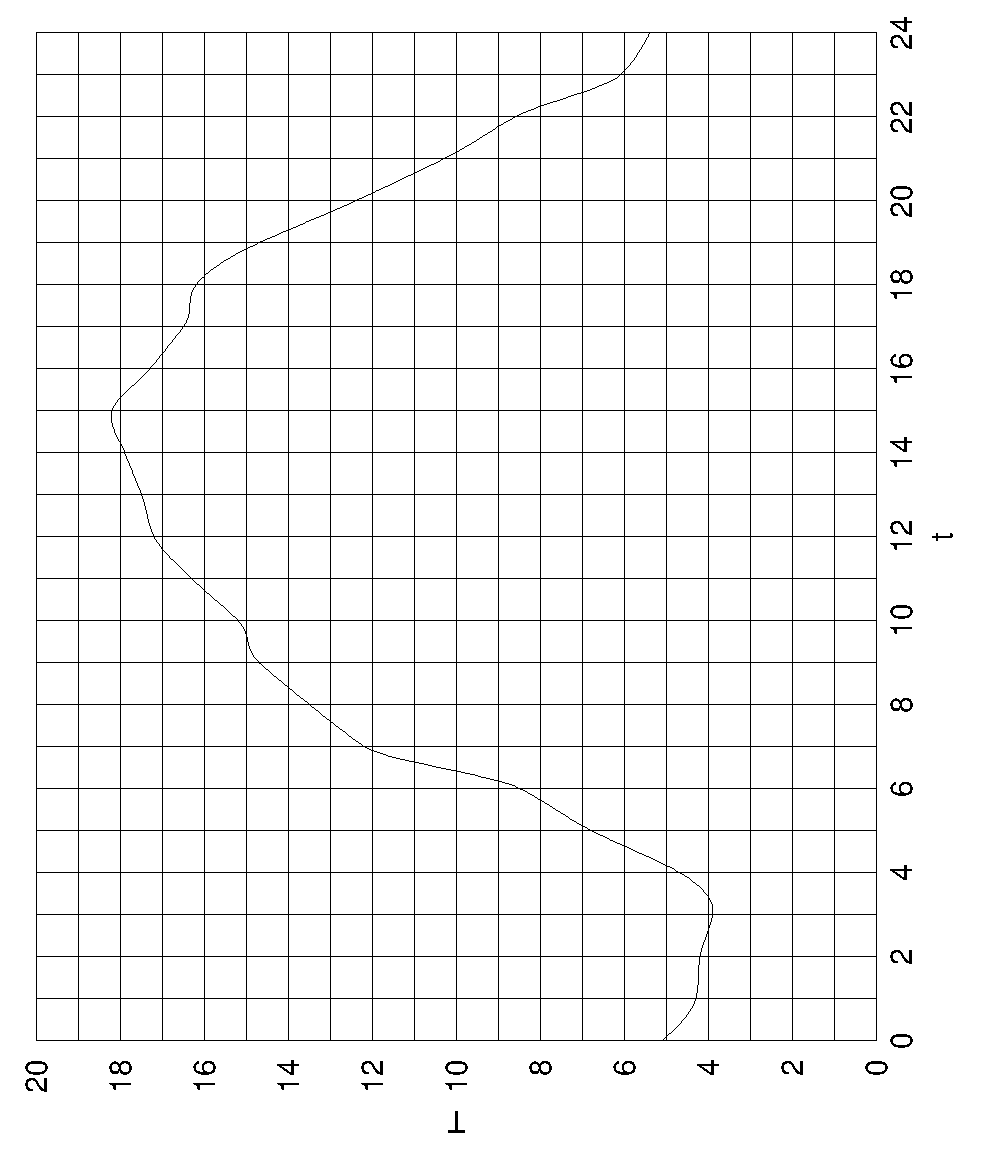
\includegraphics[angle=-90,width=0.9\columnwidth]{pictures/temp.eps}
  \caption{Temperaturverlauf innerhalb eines Tages}
  \label{fig:linfkt1:temp}
\end{figure}

\begin{figure}[b!]
  	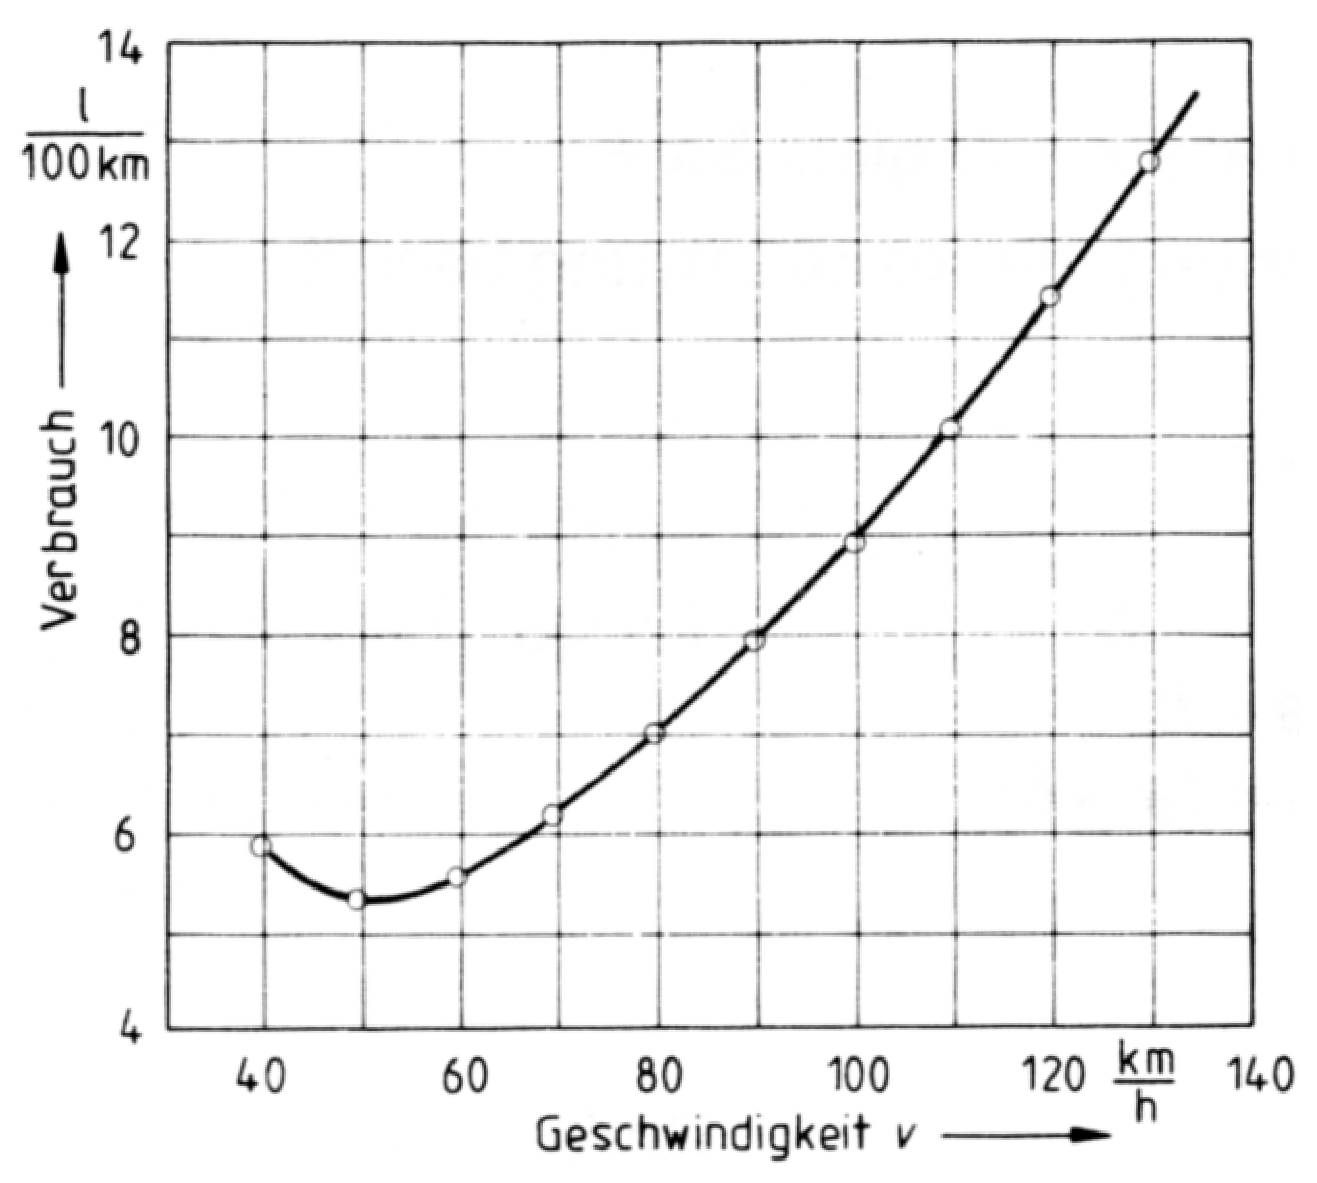
\includegraphics[width=0.9\columnwidth,bb=14 14 630 566]{pictures/treibstoff.eps}
  \caption{Treibstoffverbrauch eines Fahrzeugs als Funktion der Geschwindigkeit}
  \label{fig:linfkt1:treibstoff}
\end{figure}

Kommen wir zum H\"utchen-Beispiel zur\"uck: Wenn wir \ref{fig:linfkt1:sthut} genauer betrachten, sehen wir, dass der Weg offensichtlich gleichm\"assig mit der Zeit zunimmt.\footnote{Dabei sehen wir von der sehr kurzen Beschleunigungsphase ab, die zu Beginn der Bewegung stattfindet.} Wir k\"onnen deshalb eine Gerade durch die Punkte ziehen, welche die Bewegung gut beschreibt --- bis auf Messungenauigkeiten und allf\"allige St\"oreffekte wie Windst\"osse etc. Wir nehmen daher an, dass die vollst\"andige Bewegung zu jedem beliebigen Zeitpunkt (auch zwischen unseren Messungen) durch diese Gerade beschrieben wird. Dies ist zwar eine Idealisierung, stimmt aber recht gut.

Die Linie, die sich in der Graphik ergibt, ist der sogenannte \emph{Graph} der
Funktion. Der Graph unserer Funktion ist also eine Gerade. Eine solche
Zuordnung wird deshalb eine \emph{lineare Funktion} genannt. Der Graph k\"onnte
ebenso gut krumm sein (wenn das H\"utchen schneller oder langsamer w\"urde). D.h. nicht alle Funktionen sind linear. Die Funktionen in \ref{fig:linfkt1:temp} und \ref{fig:linfkt1:treibstoff} beispielsweise sind nicht linear. Wir besch\"aftigen uns zun\"achst aber nur mit linearen Funktionen eingehender.


\section{Steigung und Proportionalit\"at}
\label{linfkt1:steigungprop}

Der Graph unserer Funktion ist eine Gerade. Stellen wir uns vor, diese Gerade w\"are die Flanke eines Bergs. Allerdings handelt es sich um eine spezielle Bergflanke: sie immer \"uberall gleich steil, d.h. die Steigung ist immer dieselbe. Als Steigung bezeichnen wir das Verh\"altnis der H\"ohendifferenz zur Horizontaldistanz. Wenn z.B. bei einer Horizontaldistanz von 2500\unit{m} die H\"ohendifferenz 500\unit{m} betr\"agt, ist die Steigung:
\begin{displaymath}
\frac{\mathrm{H\ddot{o}hendifferenz}}{\mathrm{Horizontaldistanz}}=\frac{500\unit{m}}{2500\unit{m}}=0.2=20\%
\end{displaymath}
Das Diagramm in \ref{fig:linfkt1:sthut} zeigt aber keinen Berg, sondern die Strecke als Funktion der Zeit. Eine H\"ohendifferenz und eine Horizonaldistanz gibt es aber auch hier: es sind die Koordinaten $s$ und $t$ der einzelnen Punkte. Das Verh\"altnis $\frac{s}{t}$ ist die hier die Steigung. Wenn wir $\frac{s}{t}$ f\"ur verschiedene Punkte der Gerade berechnen, muss immer dasselbe herauskommen, weil die Gerade \"uberall gleich steil ist. In \ref{tab:linfkt1:vhut} ergibt sich allerdings nicht immer genau der gleiche Wert. Das ist klar, denn die Messpunkte liegen nicht genau auf der Geraden. W\"urden wir $\frac{s}{t}$ f\"ur Punkte berechnen, die genau auf der Geraden liegen, erg\"abe sich immer genau dasselbe Resultat. Denn die Strecken $s$ und $t$ bilden zusammen mit der Geraden jeweils ein so genanntes Steigungsdreieck, dessen Seitenverh\"altnisse (insbesondere $\frac{s}{t}$) immer gleich sind.

\begin{table}[t!]
  \centering
  \begin{tabular}{|c|c|c|}
    \hline
    t\,[s] & s\,[m] & $v=\frac{s}{t}$ [$\!\ufrac{m}{s}$] \\[0.5ex] \hline\hline
	1 & 0.86 & 0.86 \\ \hline
	2 & 1.53 & 0.77 \\ \hline
	3 & 2.34 & 0.78 \\ \hline
	4 & 3.22 & 0.81 \\ \hline
	5 & 3.89 & 0.78 \\ \hline
	6 & 4.73 & 0.79 \\ \hline
  \end{tabular}
  \caption{Das Verh\"altnis $\frac{s}{t}$ mit Hilfe der verschiedenen Messpunkte berechnet.}
  \label{tab:linfkt1:vhut}
\end{table}

Man sagt auch: Das Verh\"altnis $\frac{s}{t}$ ist konstant und schreibt:
\begin{displaymath}
\frac{s}{t}=const.
\end{displaymath}
Ein anderes Wort f\"ur \begriff{Verh\"altnis} ist \begriff{Proportion}. Wenn das Verh\"altnis zweier Gr\"ossen immer gleich ist, sagt man daher, dass sie \emph{proportional} zueinander sind. Die Strecke $s$ des H\"utchens ist proportional zur Zeit $t$.

Das Verh\"altnis der Strecke $s$ zur Zeit $t$ ist bekanntlich die Geschwindigkeit $v$ des H\"utchens ($v$ f\"ur englisch \begriff{velocity} oder franz\"osisch \begriff{vitesse}):
\begin{displaymath}
\frac{s}{t}=v
\end{displaymath}
Offenbar entspricht die Geschwindigkeit $v$ der Geradensteigung in \ref{fig:linfkt1:sthut} und bleibt immer gleich:
\begin{displaymath}
v=const.
\end{displaymath}
Auf Grund unserer Messwerte haben wir jedoch nicht immer die gleiche Geschwindigkeit erhalten (siehe \ref{tab:linfkt1:vhut}), weil sie --- wegen Messungenauigkeiten und St\"oreffekten --- nicht genau einer linearen Funktion folgen. Um aber f\"ur unsere idealisierte Funktionsgleichung einen m\"oglichst genauen Geschwindigkeitswert zu erhalten, w\"ahlen wir eine m\"oglichst lange Zeit und damit eine m\"oglichst lange Strecke:
\begin{displaymath}
v=\frac{4.73\unit{m}}{6\unit{s}}=0.79\ufrac{m}{s}
\end{displaymath}


\section{Funktionsgleichung}
\label{linfkt1:gleichung}

Unsere lineare Funktion ordnet jedem Zeitpunkt $t$ die zur\"uckgelegte Strecke $s$ des Papierh\"utchens zu. Diese Zuordnung haben wir in \ref{tab:linfkt1:hut} und in \ref{fig:linfkt1:sthut} dargestellt. Man kann aber auch zu jeder Zeit $t$ die zugeh\"orige Strecke $s$ \emph{berechnen}. Gesucht ist z.B. die Strecke nach der Zeit $t=3.5\unit{s}$. Gem\"ass der obigen Gleichung $\frac{s}{t}=v$ muss gelten:
\begin{eqnarray*}
\frac{s}{3.5\unit{s}} & = & 0.79\ufrac{m}{s} \\
s & = & 0.79\ufrac{m}{s}\cdot 3.5\unit{s}=2.8\unit{m}
\end{eqnarray*}
Nach 3.5\unit{s} ist das H\"utchen bei etwa 2.8\unit{m}. Um eine Formel zu erhalten, mit der man zu jedem beliebigen Zeitpunkt $t$ die Strecke $s$ berechnen kann, l\"osen wir die allgemeine Gleichung nach $s$ auf:
\begin{displaymath}
s = v t
\end{displaymath}
wobei immer $v=0.79\ufrac{m}{s}$ ist. Damit k\"onnen wir den ganzen Bewegungsverlauf, d.h. die ganze Funktion mit einer einzigen Gleichung beschreiben, was sehr effizient ist. Deshalb nennen wir $s=vt$ die \emph{Funktionsgleichung}. Mit ihr k\"onnen wir jedem $t$ das zugeh\"orige $s$ zuordnen, indem wir $t$ mit $v=0.79\ufrac{m}{s}$ multiplizieren. Der Faktor $v$, den wir mit $t$ multiplizieren, ist immer gleich, weil $s$ und $t$ proportional zueinander sind. Deshalb nennen wir $v$ auch \emph{Proportionalit\"atsfaktor}.

Nun haben wir drei M\"oglichkeiten, eine Funktion darzustellen: durch eine Tabelle, den Graphen oder die Funktionsgleichung. Wenn wir jedoch nicht nur jeder Sekunde, sondern jedem beliebigen Zeitpunkt eine Strecke zuordnen wollen, liefert die Tabelle nur eine unvollst\"andige Darstellung. Der Graph hingegen ist l\"uckenlos. Er ist aber nicht beliebig genau und er ist begrenzt, w\"ahrend die Funktionsgleichung zu jedem beliebigen $t$ das $s$ exakt liefert (zumindest theoretisch).

Zudem ist die Funktionsgleichung die kompakteste Art, die Funktion zu beschreiben, und mit Hilfe der Algebra liefert sie uns Antworten auf viele Fragen: Durch Umformung erhalten wir z.B. eine Formel, mit der wir die Zeit berechnen k\"onnen, nach der das H\"utchen einen bestimmten Weg zur\"uckgelegt hat:
\begin{displaymath}
t = \frac{s}{v}
\end{displaymath}
Wann hat das H\"utchen die Strecke $s=3.7\unit{m}$ zur\"uckgelegt? Nach
\begin{displaymath}
t = \frac{3.7\unit{m}}{0.79\ufrac{m}{s}}=4.7\unit{s}
\end{displaymath}
Zum Rechnen ist also die Funktionsgleichung sehr gut. Der Graph hingegen ist sehr anschaulich. Wir werden daher beide Mittel --- m\"oglichst geschickt --- einsetzen. Tabellen werden wir allenfalls erstellen, um mit ihrer Hilfe Funktionsgraphen zu zeichnen.

Allerdings k\"onnen wir nicht f\"ur jede Funktion eine (mehr oder weniger einfache) Funktionsgleichung finden. F\"ur die Funktion in \ref{fig:linfkt1:temp} beispielsweise wird das wohl kaum gelingen. Dann bleiben uns nur noch der Graph und die Tabelle. Zun\"achst betrachten wir aber ohnehin nur linare Funktionen. Und dazu geh\"ort die Funktion in \ref{fig:linfkt1:temp} nicht.

\begin{figure}[t!]
\centering
\psfrag{v1}[][][2]{$v_1$} \psfrag{v2}[][][2]{$v_2$} \psfrag{v3}[][][2]{$v_3$}
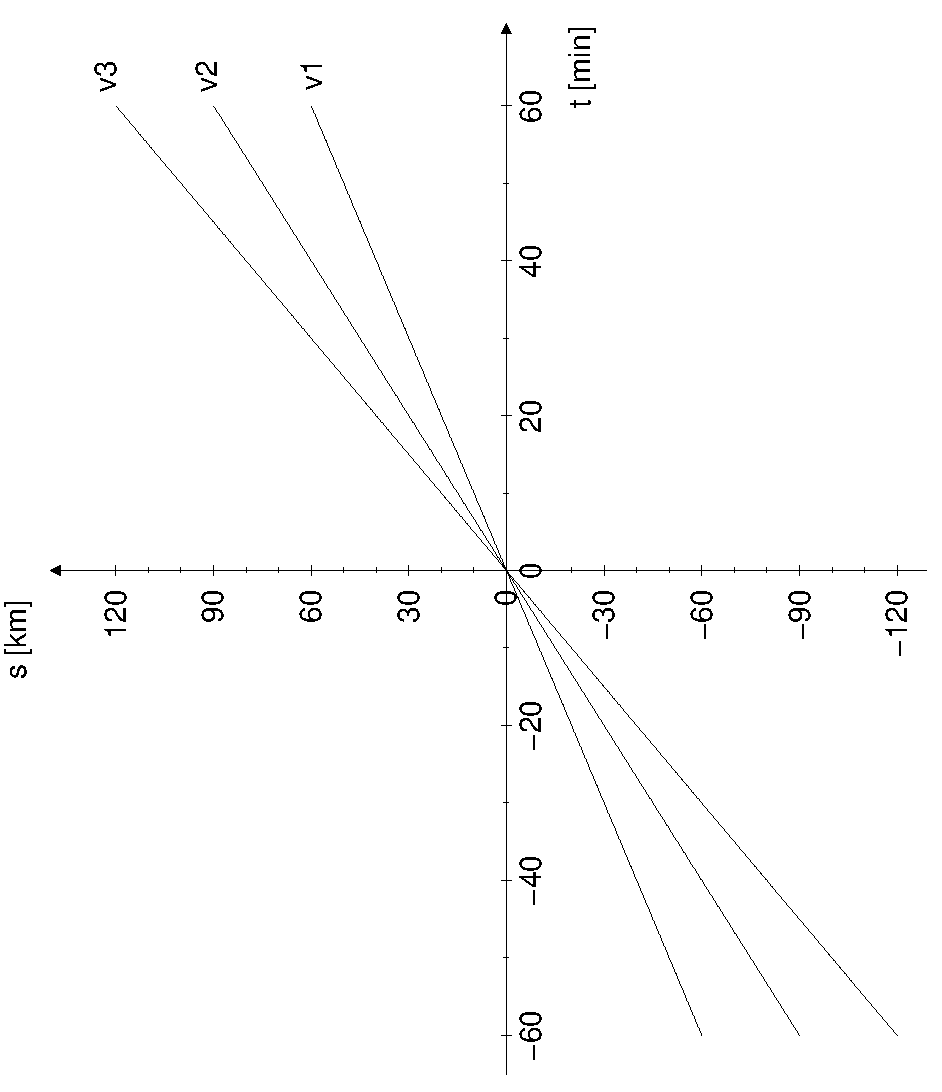
\includegraphics[angle=-90,width=0.9\columnwidth]{pictures/dreizug.eps}
\caption{Die Graphen von drei Z\"ugen mit den Geschwindigkeiten $v_1=60\ufrac{km}{h}$, $v_2=90\ufrac{km}{h}$ und $v_3=120\ufrac{km}{h}$. Wir haben die Bewegungen auch vor den Zeitpunkt $t=0$ zur\"uckverfolgt.}
\label{fig:linfkt1:dreizug}
\end{figure}

\section{Proportionalit\"atsfaktor bzw. Steigung variieren}
\label{linfkt1:steigung}

Mit der Funktionsgleichung $s=vt$ k\"onnen wir nicht nur die Bewegung unseres H\"utchens beschreiben, sondern ebenso gut die Bewegung eines Zuges darstellen, der sich mit konstanter Geschwindigkeit bewegt. Die mathematische Beschreibung ist --- wie immer --- sehr allgemein verwendbar. Allerdings ist ein Zug in der Regel schneller. Zudem k\"onnen Z\"uge verschiedene Geschwindigkeiten $v$ haben. Wie \"aussert sich das im Graphen? Im Diagramm von \ref{fig:linfkt1:dreizug} sind die Bewegungen dreier Z\"uge dargestellt, die sich mit konstanten Geschwindigkeiten von $v_1=60\ufrac{km}{h}$, $v_2=90\ufrac{km}{h}$ und $v_3=120\ufrac{km}{h}$ bewegen. Wir sehen: Je schneller der Zug ist, desto steiler ist die Gerade. Das ist klar: In Abschnitt \ref{linfkt1:steigungprop} haben wir gesehen, dass die Geschwindigkeit der Geradensteigung im Weg-Zeit-Diagramm entspricht.



\section{Verallgemeinerung}
\label{linfkt1:allg}

\subsection{Alles mit x und y}
\label{linfkt1:allg:xy}

Die Eigenschaften linearer Funktionen k\"onnen wir in der Mathematik ganz allgemein studieren. Das Wissen, das wir dabei erwerben, k\"onnen wir auf alle linearen Funktionen anwenden, unabh\"angig von der konkreten Situation. Das ist die St\"arke der Mathematik. Der Preis, den wir daf\"ur bezahlen, ist die Abstraktion. Bei unseren allgemeinen Betrachtungen sprechen wir nicht \"uber konkrete Gr\"ossen, wie die Zeit $t$ und die Strecke $s$, sondern \"uber abstrakte Gr\"ossen, f\"ur die wir in der Regel die Variablen $x$ und $y$ verwenden, wenn uns nichts Kl\"ugeres einf\"allt. Und zwar \"ubernimmt das $x$ die Rolle des $t$ und das $y$ jene des $s$. D.h es soll jedem $x$ ein $y$ zugeordnet werden. Im Graphen tragen wir dementsprechend das $x$ waagrecht auf und das $y$ senkrecht (siehe \ref{fig:linfkt1:steigungen}). Wenn $x$ und $y$ proportional zueinander sind, d.h. wenn ihr Verh\"altnis immer gleich ist, gilt:
\begin{displaymath}
  a = \frac{y}{x}=const.
\end{displaymath}
Dabei steht der \emph{Proportionalit\"atsfaktor} $a$ f\"ur eine bestimmte Zahl, die sich nicht ver\"andert. Daraus ergibt sich die Funktionsgleichung, mit der wir zu jedem $x$ das zugeh\"orige $y$ berechnen k\"onnen:
\begin{displaymath}
  y = ax
\end{displaymath}
Jede solche Gleichung beschreibt eine Gerade, die durch den Koordinaten-Nullpunkt\footnote{Der Nullpunkt des Koordinatensystems wird auch \emph{Koordinaten-Ursprung} oder nur \emph{Ursprung} genannt.} verl\"auft, denn f\"ur $x=0$ ist gem\"ass obiger Gleichung immer auch $y=0$. Die Steigung dieser Geraden ist $a$.


\subsection{Den Graphen zeichnen}
\label{linfkt1:allg:graph}

Ist umgekehrt die Steigung $a$ bekannt, k\"onnen wir mit Hilfe der Funktionsgleichung die Gerade (d.h. den Graphen) zeichnen. Dabei k\"onnen wir eine Tabelle mit den $x$- und $y$-Werten erstellen (\"ahnlich wie \ref{tab:linfkt1:hut}), indem wir zu jedem $x$ mit Hilfe der Funktionslgleichung des zugeh\"orige $y$ berechnen. Dann zeichnen wir die Punkte in ein Koordinatensystem ein. Schliesslich verbinden wir die Punkte.

Weil der Graph einer linearen Funktion eine Gerade ist, reichen in diesem Fall allerdings zwei Punkte. Wenn $x$ und $y$ proportional zueinander sind, geht diese Gerade sogar durch den Koordinaten-Nullpunkt (siehe oben). D.h. es braucht nur noch einen zweiten Punkt.

\begin{figure}[b!]
\centering
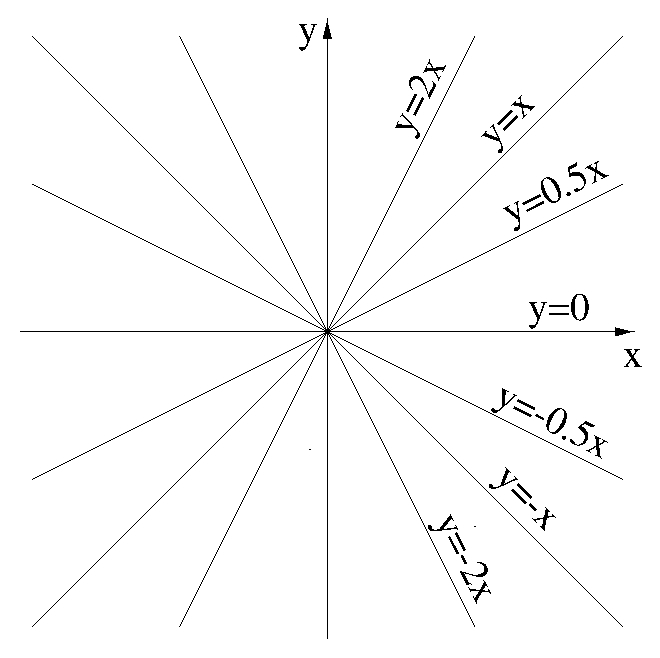
\includegraphics[width=0.8\columnwidth]{pictures/steigungen.eps}
\caption{Geraden mit verschiedenen Steigungen: Positive Steigung ($a>0$) bedeutet Steigen, negative Steigung ($a<0$) bedeutet Fallen. Die $x$-Achse entspricht der Funktion $y=0$, f\"ur welche die Steigung Null ist.}
\label{fig:linfkt1:steigungen}
\end{figure}

In \ref{fig:linfkt1:steigungen} sind die Graphen verschiedener linearer Funktionen gezeichnet. Sie haben verschiedene Steigungen: Die Gerade zur Gleichung $y=2x$ hat z.B. die Steigung 2: die H\"ohendifferenz ist immer doppelt so gross wie die Horizontaldistanz. Bei der Geraden $y=0.5x$ ist die Steigung 0.5: Die H\"ohendifferenz ist immer halb so gross wie die Horizontaldistanz.

Wenn die Steigung negativ ist, heisst das, dass wir um eine negative H\"ohe steigen, wenn $x$ zunimmt (von links nach rechts). D.h. die Gerade f\"allt. (Wenn $x$ positiv ist, ist $y$ negativ --- und umgekehrt.)


\section{Punkte im Koordinatensystem}
\label{linfkt1:punkte}

Jedes $x$-$y$-Paar k\"onnen wir in einer k\"urzeren Schreibweise zusammenfassen: Z.B. wird das Paar $x=3$ und $y=9$ so dargestellt:\footnote{Manchmal wird anstelle des senkrechten Strichs auch ein Komma oder ein Strichpunkt gesetzt: (3,5) oder (3;5).} $(3|9)$. Allgemein fassen wir ein $x$-$y$-Paar wie folgt zusammen:
\begin{displaymath}
  (x|y)
\end{displaymath}
Jedes solche Paar entspricht einem Punkt im Koordinatensystem. Alle $(x|y)$-Punkte, welche die Funktionsgleichung erf\"ullen, bilden den Graphen.

Wenn wir einem bestimmten Punkt im Koordinatensystem z.B. den Namen $P$ geben wollen, schreiben wir diesen Namen vor seine Koordinaten:
\begin{displaymath}
  P(x|y)
\end{displaymath}
z.B. $P(3|9)$.


%\section*{Lernziele \thesection}
{\settowidth{\labelwidth}{\labelitemi}
\setlength{\leftmargini}{\labelwidth} \addtolength{\leftmargini}{\labelsep}
%Sie k\"onnen\dots
%\begin{itemize}
%\item \dots erkl\"aren, was eine Funktion ist und wie man sie darstellen kann, wobei Sie die entsprechenden Begriffe und Sprechweisen verwenden (\begriff{Graph}, \begriff{Funktionsgleichung}, \rede{\ldots ist eine Funktion von\,\dots})
%\item \dots erkl\"aren, was eine \emph{lineare} Funktion ist
%\item \dots eine lineare Funktion, deren Graph durch den Koordinaten-Nullpunkt geht, allgemein algebraisch beschreiben
%\item \dots erkl\"aren, was die Steigung einer Geraden ist
%\item \dots zu jeder gegebenen linearen Funktionsgleichung die Steigung angeben
%\item \dots den Graphen einer linearen Funktion vom Typ $y=ax$ zeichnen, wenn $a$ gegeben ist.
%\item \dots die Steigung und damit die Funktionsgleichung $y=ax$ bestimmen, wenn der Graph oder auch nur ein Punkt der Funktion gegeben ist (zus\"atzlich zum Koordinaten-Nullpunkt)
%\item \dots den Begriff \begriff{Proportionalit\"at} (\begriff{proportional}) erkl\"aren und anwenden
%\item \dots die Koordinaten von Punkten aufschreiben
%\end{itemize}}




\section*{Aufgaben}
{\settowidth{\labelwidth}{9.9}
\setlength{\leftmargini}{\labelwidth} \addtolength{\leftmargini}{\labelsep}
\renewcommand{\labelenumi}{\thesection.\arabic{enumi}}
\begin{enumerate}

\item \label{aufg:linfkt1:stoff} Ein Kleiderstoff kostet Fr.~12.50 pro Meter. Schreiben Sie die Funktionsgleichung auf, die den Zusammenhang zwischen L\"ange und Preis darstellt, und tragen Sie den Graphen in ein Koordinatensystem ein. Lesen Sie daran die Preise f\"ur folgende L\"angen ab: 4\unit{m}, 2.5\unit{m}, 7\unit{m}, 5.4\unit{m}.

\begin{figure}[t!]
\centering
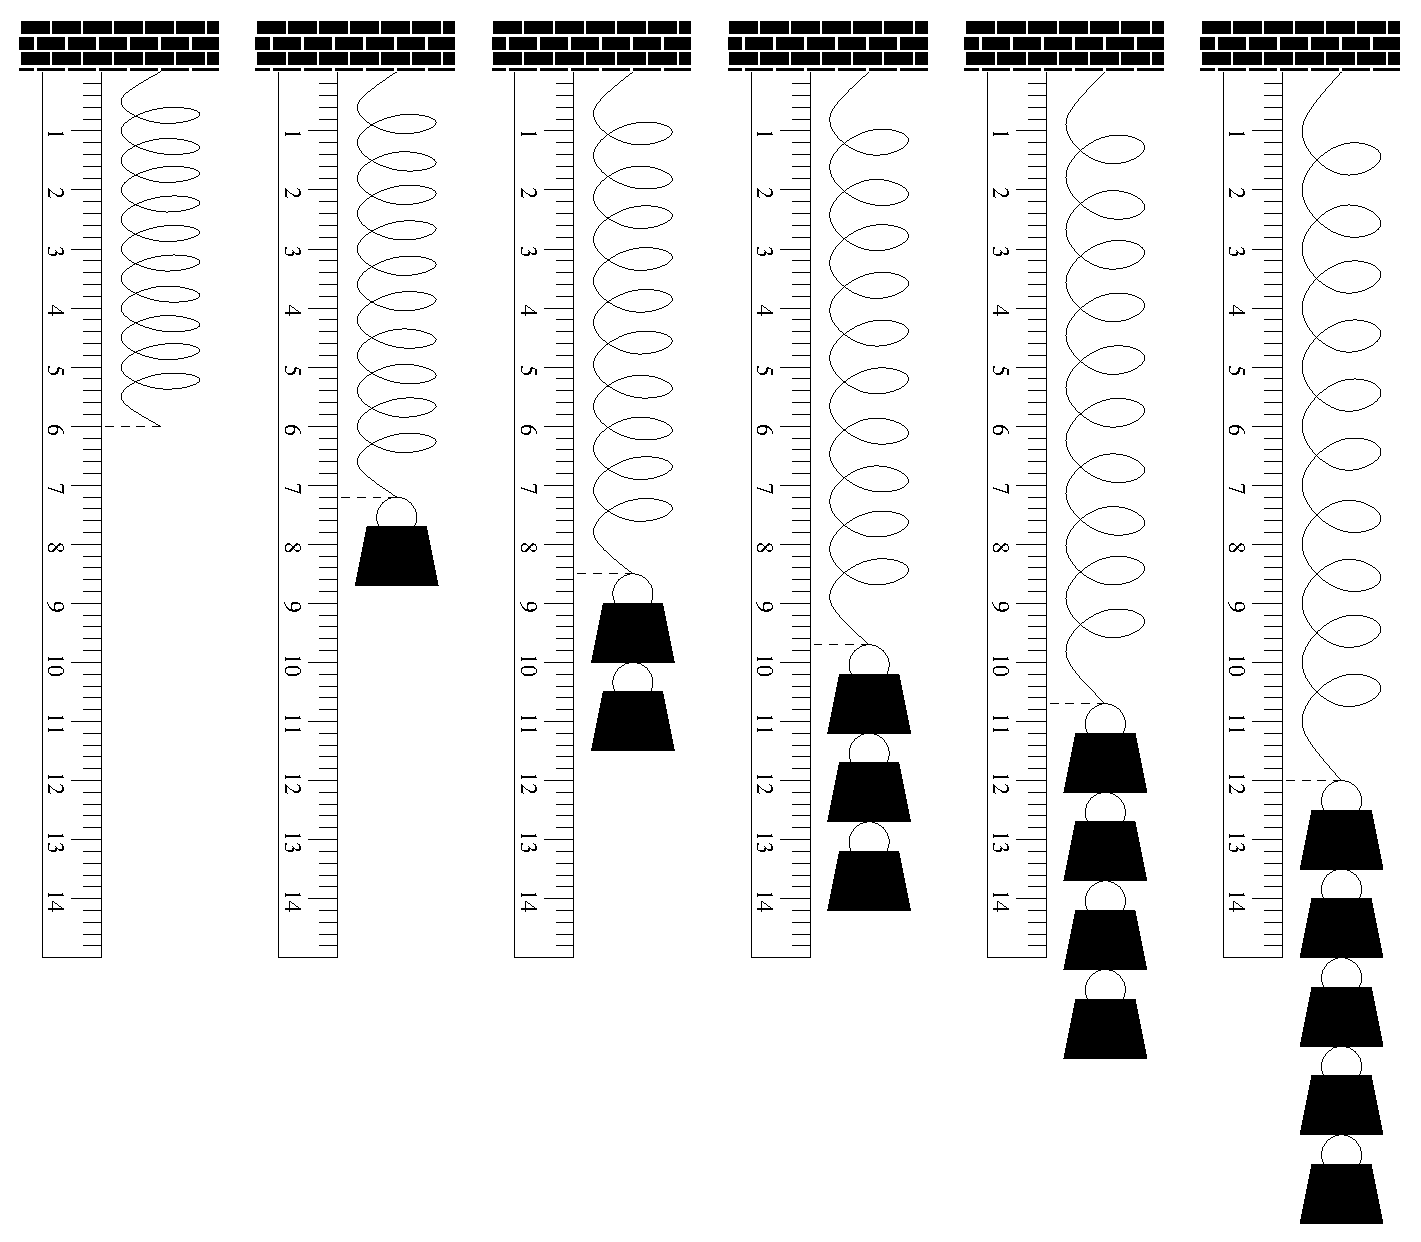
\includegraphics[width=\columnwidth]{pictures/feder.eps}
\caption{Verl\"angerung einer Feder durch angeh\"angte Gewichtssteine: Auf dem Massstab sind die L\"angen in cm angegeben.}
\label{fig:linfkt1:feder}
\end{figure}

\item An eine Feder werden nach und nach mehr Gewichte geh\"angt, wobei sich die Feder immer mehr ausdehnt (siehe \ref{fig:linfkt1:feder}). Jeder der angeh\"angten Gewichtssteine hat eine Masse von 2\unit{kg}. Betrachten Sie im Folgenden die Feder-Verl\"angerung als Funktion der (Gewichts-)Kraft.\footnote{Beachten Sie: Die \emph{Verl\"angerung} ist der Betrag, um den die Feder gegen\"uber ihrem entspannten Zustand \emph{l\"anger} wird.} Rechnen Sie dabei mit dem Ortsfaktor $g=10\ufrac{N}{kg}$.
\begin{enumerate}
\item\label{aufg:linfkt1:federgraph} Zeichnen Sie den Graphen der oben erw\"ahnten Funktion.
\item Beschreiben Sie den beobachteten Zusammenhang zwischen der Verl\"angerung und der Kraft in Worten. Ist dieser Zusammenhang normal f\"ur eine Feder?
\item\label{aufg:linfkt1:federgl} Geben Sie die Funktionsgleichung an.
\item\label{aufg:linfkt1:federbsp} Um wie viel verl\"angert sich die Feder (gegen\"uber dem entspannten Zustand) wenn eine Kraft von 72\unit{N} auf sie wirkt?
\end{enumerate}

\item Vier Z\"uge bewegen sich mit den konstanten Geschwindigkeiten $v_1=42\ufrac{km}{h}$, $v_2=98\ufrac{km}{h}$, $v_3=86\ufrac{km}{h}$, $v_4=107\ufrac{km}{h}$. Tragen Sie alle Bewegungen \"uber eine Stunde hinweg in ein Weg-Zeit-Diagramm ein.

\item Zeichnen Sie die Geraden mit folgenden Funktionsgleichungen in ein Koordinatensystem:
  \begin{enumerate}
  \item $y=1.5x$
  \item $y=-0.8x$
  \item $y=-\frac{1}{2}x$
  \item $y=\frac{5}{3}x$
  \item $y=-\frac{4}{3}x$
  \end{enumerate}

\item Zeichnen Sie jeweils eine Gerade mit der angegebenen Steigung, die den Nullpunkt des Koordinatensystems durchquert und geben Sie die zugeh\"orige Funktionsgleichung an:
  \begin{enumerate}
  \item Steigung: $\displaystyle -3$
  \item Steigung: $\displaystyle \frac{1}{5}$
  \item Steigung: $\displaystyle -\frac{3}{5}$
  \item Steigung: $\displaystyle -\frac{7}{4}$
  \end{enumerate}


\item Jede der folgenden Wertetabellen enth\"alt zwei Punkte, die zu einer linearen Funktion geh\"oren. Geben Sie jeweils die Funktionsgleichung an.
  \begin{enumerate}
  \item 
    \begin{tabular}{|c|c|} 
      \hline 
      x & y \\ \hline\hline
      0 & 0 \\ \hline
      1 & --3 \\ \hline
    \end{tabular}
  \item 
    \begin{tabular}{|c|c|} 
      \hline 
      x & y \\ \hline\hline
      0 & 0 \\ \hline
      1 & 4.3 \\ \hline
    \end{tabular}
  \item 
    \begin{tabular}{|c|c|} 
      \hline 
      x & y \\ \hline\hline
      0 & 0 \\ \hline
      1 & --1 \\ \hline
    \end{tabular}
  \item 
    \begin{tabular}{|c|c|} 
      \hline 
      x & y \\ \hline\hline
      0 & 0 \\ \hline
      1 & 0 \\ \hline
    \end{tabular}
  \item 
    \begin{tabular}{|c|c|} 
      \hline 
      x & y \\ \hline\hline
      0 & 0 \\ \hline
      2 & 5 \\ \hline
    \end{tabular}
  \item 
    \begin{tabular}{|c|c|} 
      \hline 
      x & y \\ \hline\hline
      0 & 0 \\ \hline
      1.5 & --3 \\ \hline
    \end{tabular}
  \end{enumerate}

\item Bestimmen Sie die Steigung der Geraden, welche durch den Ursprung geht und durch den jeweils angegebenen Punkt, und schreiben Sie die zugeh\"orige Funktionsgleichung auf:
  \begin{enumerate}
  \item $(1|-5)$
  \item $(1|0.5)$
  \item $(3|2)$
  \item $(4|0)$
  \item $(0.5|2)$
  \item $(4|-3)$
  \item $(-1|2)$
  \item $(-1|-2.5)$
  \item $(-3|2)$
  \item $(-3|-4)$
  \end{enumerate}


\item Zeichnen und vergleichen Sie jeweils die beiden Geraden. Was stellen Sie fest?
  \begin{enumerate}
  \item $y=2x$ und $y=-\frac{1}{2}x$
  \item $y=\frac{1}{3}x$ und $y=-3x$
  \item $y=-\frac{2}{3}x$ und $y=\frac{3}{2}x$
  \item $y=-\frac{5}{2}x$ und $y=\frac{2}{5}x$
  \end{enumerate}

\end{enumerate}}


\section*{L\"osungen}
{\settowidth{\labelwidth}{L9.9}
\setlength{\leftmargini}{\labelwidth} \addtolength{\leftmargini}{\labelsep}
\renewcommand{\labelenumi}{L\thesection.\arabic{enumi}}
\begin{enumerate}

\item $l$: L\"ange, $p$: Preis
  \begin{displaymath}
    \result{p=12.5\ufrac{Fr.}{m} \cdot l}
  \end{displaymath}

\begin{center}
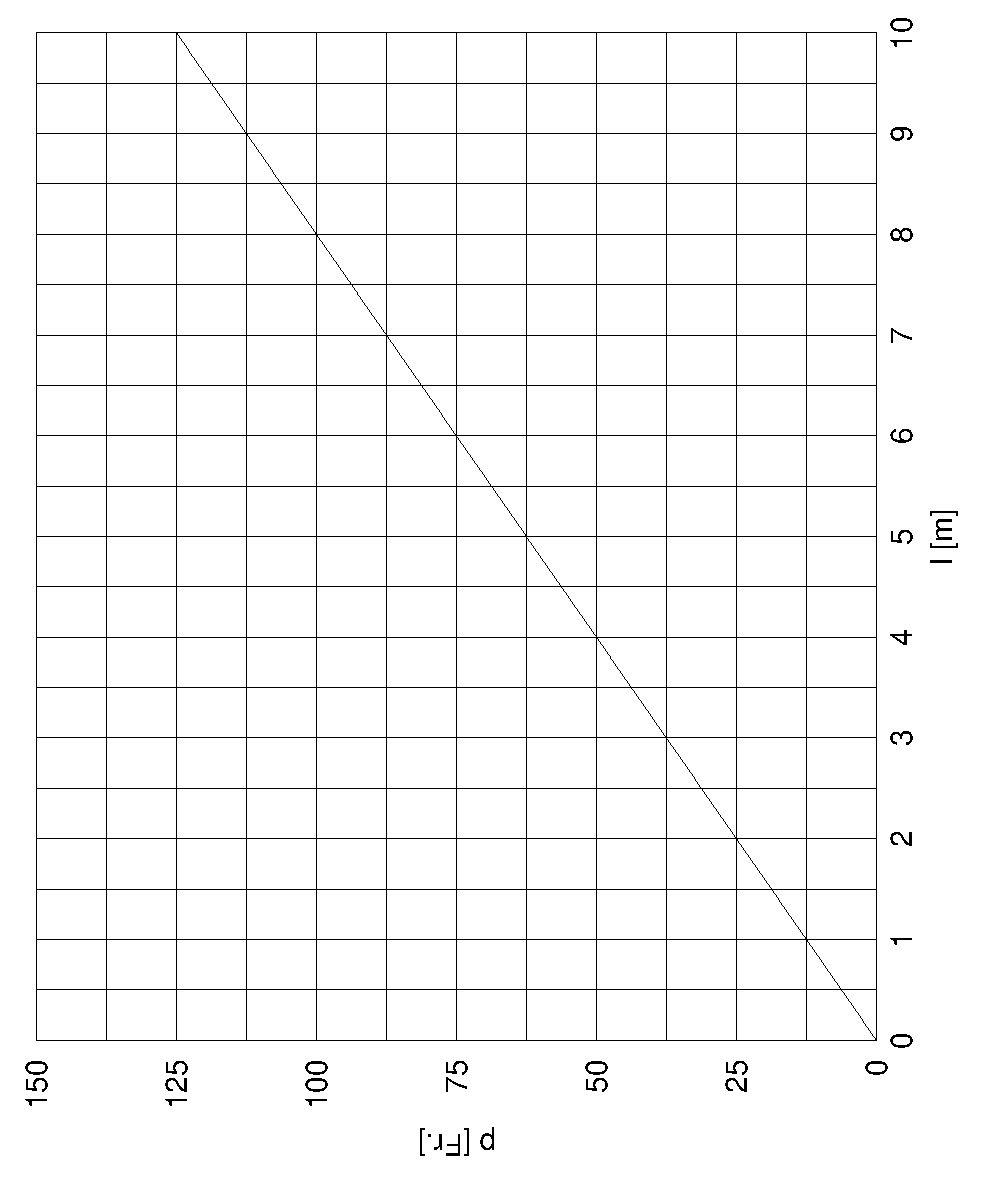
\includegraphics[angle=-90,width=\linewidth]{pictures/stoff.eps}
\end{center}

4\unit{m}: $\result{50\unit{Fr.}}$; 2.5\unit{m}: $\result{31.25\unit{Fr.}}$; 7\unit{m}: $\result{87.50\unit{Fr.}}$; 5.4\unit{m}: $\result{67.50\unit{Fr.}}$

\item Ein Gewichtsst\"uck hat die Masse von $m=2\unit{kg}$. Seine Gewichtskraft ist $F=mg=2\unit{kg}\cdot 10\ufrac{N}{kg}=20\unit{N}$
\begin{enumerate}
\item \mbox{}\vspace*{-2\baselineskip}
\begin{center}
\begin{minipage}{4cm}
\centering
\begin{tabular}{|c|c|}
\hline
$F$\,[N] & $\Delta l$\,[cm] \\ \hline\hline
0 & 0 \\ \hline
20 & 1.2 \\ \hline
40 & 2.5 \\ \hline
60 & 3.7 \\ \hline
80 & 4.7 \\ \hline
100 & 6 \\ \hline
\end{tabular}
\end{minipage}
\hspace{2cm}
\begin{minipage}{6cm}
\psfrag{dl [cm]}[][][0.8]{$\Delta l$ [cm]}
\includegraphics[width=\linewidth]{pictures/flfeder.eps}
\end{minipage}
\end{center}
Die Gerade wurde so zwischen den Punkten hindurchgezeichnet, dass sie m\"oglichst wenig von diesen abweicht.

\item Der Zusammenhang zwischen der Kraft und der Verl\"angerung ist linear. Die Verl\"angerung ist proportional zur Kraft. D.h., wenn die Kraft z.B. verdoppelt wird, so wird auch die Verl\"angerung doppelt so gross. Dieser Zusammenhang ist normal f\"ur eine Feder, so lange sie nicht \"uberdehnt wird.
\item Das Verh\"altnis von Kraft und Verl\"angerung bleibt konstant und ist gleich der Federkonstanten (hookesches Gesetz):
  \begin{eqnarray*}
    D & = & \frac{F}{\Delta l} \\
    D\Delta l & = & F \\
    \Delta l & = & \frac{1}{D}F
  \end{eqnarray*}
Die Proportionalit\"atskonstante ist $\frac{1}{D}$, d.h. der Kehrwert der Federkonstanten. W\"urde man die Kraft als Funktion der Verl\"angerung betrachten, w\"urde die Funktionsgleichung $F=D\Delta l$ lauten, d.h. die Proportionalit\"atskonstante w\"are die Federkonstante $D$ selbst.
  
Die Federkonstante berechnen wir aus den gr\"ossten Werten (weil dann die Ungenauigkeiten im Verh\"altnis zu den gemessenen Werten am kleinsten sind):
\begin{eqnarray*}
  D & = & \frac{100\unit{N}}{6\unit{cm}}=17\ufrac{N}{cm} \\
  \Delta l & = & \frac{1}{17}\ufrac{cm}{N}\cdot F
\end{eqnarray*}
\item $F=72\unit{N}$: $\Delta l=4.2\unit{cm}$
\end{enumerate}



\item
\begin{center}
\psfrag{v1}[][][2]{$v_1$} \psfrag{v2}[][][2]{$v_2$} \psfrag{v3}[][][2]{$v_3$} \psfrag{v4}[][][2]{$v_4$}
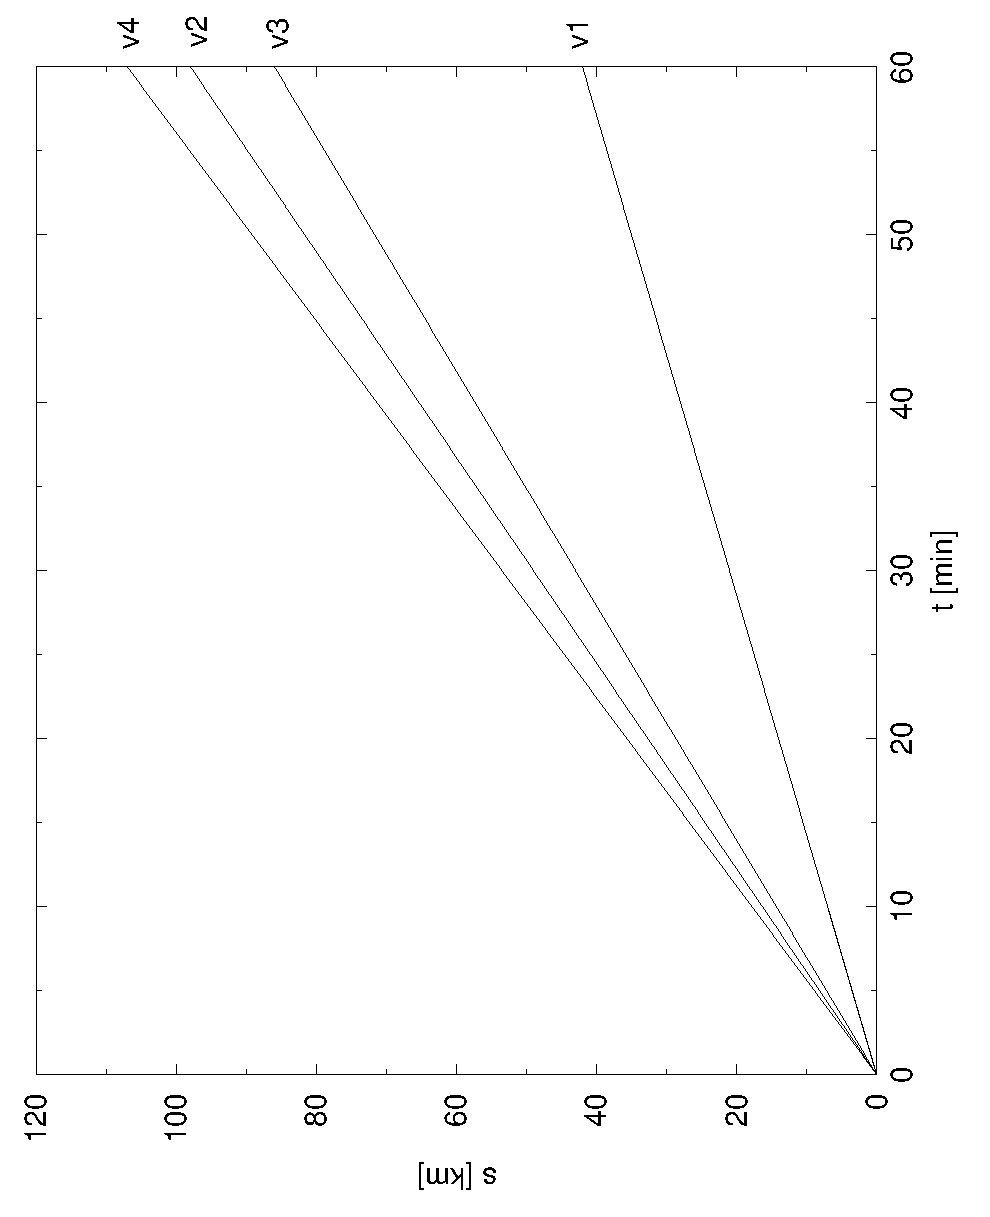
\includegraphics[angle=-90,width=\linewidth]{pictures/vierzug.eps}
\end{center}

\item \mbox{}\vspace*{-\baselineskip}
\begin{center}
\includegraphics[width=0.9\linewidth]{pictures/geraden1.eps}
\end{center}

\item
  \begin{enumerate}
  \item $\displaystyle y=-3x$
  \item $\displaystyle y=\frac{1}{5}x$
  \item $\displaystyle y=-\frac{3}{5}x$
  \item $\displaystyle y=-\frac{7}{4}x$
  \end{enumerate}

\begin{center}
\includegraphics[width=0.9\linewidth]{pictures/geraden2.eps}
\end{center}

\item
  \begin{enumerate}
  \item $\displaystyle a=\frac{y}{x}=\frac{-3}{1}=-3 \;\rightarrow\; \result{y=-3x}$
  \item $\displaystyle a=4.3 \quad\rightarrow\quad \result{y=4.3x}$
  \item $\displaystyle a=-1 \quad\rightarrow\quad \result{y=-x}$
  \item $\displaystyle a=0 \quad\rightarrow\quad \result{y=0}$
  \item $\displaystyle a=\frac{y}{x}=\frac{5}{2} \;\rightarrow\; \result{y=\frac{5}{2}x}$
  \item $\displaystyle a=\frac{-3}{1.5}=-2 \quad\rightarrow\quad \result{y=-2x}$
  \end{enumerate}

\item
  \begin{enumerate}
  \item $\displaystyle a=\frac{y}{x}=\frac{-5}{1}=-5 \;\rightarrow\; \result{y=-5x}$
  \item $\displaystyle a=0.5 \quad\rightarrow\quad \result{y=0.5x}$
  \item $\displaystyle a=\frac{y}{x}=\frac{2}{3} \;\rightarrow\; \result{y=\frac{2}{3}x}$
  \item $\displaystyle a=\frac{0}{4}=0 \quad\rightarrow\quad \result{y=0}$
  \item $\displaystyle a=\frac{2}{0.5}=4 \quad\rightarrow\quad \result{y=4x}$
  \item $\displaystyle a=-\frac{3}{4} \quad\rightarrow\quad \result{y=-\frac{3}{4}x}$
  \item $\displaystyle a=-2 \quad\rightarrow\quad \result{y=-2x}$
  \item $\displaystyle a=2.5 \quad\rightarrow\quad \result{y=2.5x}$
  \item $\displaystyle a=-\frac{2}{3} \quad\rightarrow\quad \result{y=-\frac{2}{3}x}$
  \item $\displaystyle a=\frac{4}{3} \quad\rightarrow\quad \result{y=\frac{4}{3}x}$
  \end{enumerate}

\item \mbox{}\vspace*{-2\baselineskip}
\begin{center}
\includegraphics[angle=-90,width=\linewidth]{pictures/perp.eps}
\end{center}
Die Geraden stehen jeweils senkrecht zueinander. Allgemein kann man sagen, dass zwei Geraden senkrecht zueinander stehen, wenn das Produkt ihrer Steigungen $-1$ ist:
\begin{displaymath}
  a_1 a_2 = -1
\end{displaymath}

\end{enumerate}}

\clearpage

Wir haben die linearen Funktionen kennen gelernt. Dabei haben wir uns f\"ur den Anfang allerdings auf Funktionen beschr\"ankt, deren Graphen durch den Nullpunkt des Koordinatensystems gehen. Linear sind jedoch alle Funktionen, deren Graphen Geraden sind, ob sie den Koordinaten-Nullpunkt durchqueren oder nicht. In diesem Kapitel betrachten wir deshalb beliebige lineare Funktionen.

\section{Das H\"utchen startet nicht bei Null}
\label{linfkt2:was}

In einem vorangegangenem Kapitel haben wir die Bewegung eines fallenden H\"utchens betrachtet. Dabei haben wir das H\"utchen der Wand entlang fallen gelassen. Damit wir laufend sehen, wo sich das H\"utchen befindet, k\"onnten wir den Massstab an die Wand montieren, an dem wir jederzeit den Ort des H\"utchens ablesen k\"onnen.

Die Bewegung haben wir als lineare Funktion beschrieben. Graphisch haben wir diese Funktion im Weg-Zeit-Diagramm dargestellt. Dort hat sich eine Gerade ergeben. Und zwar verlief diese Gerade durch den Koordinaten-Ursprung. Das war deshalb so, weil wir den Massstab so angelegt haben, dass zum Zeitpunkt $t=0$ das H\"utchen bei $s=0$ startet. 

Wenn wir den Massstab an die Wand montieren, kann es auch sein, dass das H\"utchen zur Zeit $t=0$ gar nicht am Anfang des Massstabs startet, sondern bereits eine bestimmte Strecke von dort entfernt ist. Was \"andert sich dann?

Sagen wir, das H\"utchen startet z.B. zur Zeit $t=0$ bei der Streckenmarkierung $s_0=1.2\unit{m}$. Dann verl\"auft die Bewegung genau gleich, nur dass das H\"utchen zu jedem Zeitpunkt um 1.2\unit{m} weiter ist als vorher. Anstelle der Messwerte von \ref{tab:linfkt1:hut} ergeben sich dann jene in \ref{tab:linfkt2:huts0}.

\begin{table}[b!]
\centering
\begin{tabular}{|c|c|}
\hline
$t$\,[s] & $s$\,[m] \\ \hline\hline
0 & 1.20 \\ \hline
1 & 2.06 \\ \hline
2 & 2.73 \\ \hline
3 & 3.54 \\ \hline
4 & 4.42 \\ \hline
5 & 5.09 \\ \hline
6 & 5.93 \\ \hline
\end{tabular}
\caption{Das fallende Papierh\"utchen startet zur Zeit $t=0$ bei $s=1.2\unit{m}$.}
\label{tab:linfkt2:huts0}
\end{table}  

Alle Werte sind um 1.2\unit{m} gr\"osser. Graphisch ist das in \ref{fig:linfkt2:sthuts0} dargestellt.

\begin{figure}[b!]
  \centering
  \psfrag{s0}[][][1]{$s_0$}
  \includegraphics[width=\columnwidth]{pictures/sthuts0.eps}
  \caption{Das Weg-Zeit-Diagramm eines H\"utchens, das zur Zeit $t=0$ nicht bei $s=0$ startet, sondern bei $s_0=1.2\unit{m}$.}
  \label{fig:linfkt2:sthuts}
\end{figure}

Wir sehen, dass die Gerade, welche die Bewegung beschreibt, einfach um den Wert $s_0=1.2\unit{m}$ nach oben verschoben ist. Wir haben also nicht mehr eine Gerade, die durch den Koordinaten-Ursprung geht, wie es in Kapitel \ref{linfkt1} der Fall war. Dort hat sich folgende Funktionsgleichung ergeben, mit der zu jedem Zeitpunkt $t$ der Ort $s$ berechnet werden kann:
\begin{displaymath}
  s = v t\;,
\end{displaymath}
wobei die Geschwindigkeit einen festen Wert $\left(v=0.79\ufrac{m}{s}\right)$ hat. Wenn das H\"utchen aber bei $s_0=1.2\unit{m}$ startet, ist die Strecke zu jedem Zeitpunkt um so viel gr\"osser als vorher. Deshalb ergibt sich folgende Funktionsgleichung:
\begin{displaymath}
  s = v t + s_0
\end{displaymath}
oder mit den oben angegebenen Daten:
\begin{displaymath}
  s = 0.79\ufrac{m}{s}\cdot t + 1.2\unit{m}
\end{displaymath}
Zum Zeitpunkt $t=0$ ist das H\"utchen nach dieser Gleichung tats\"achlich am Ort $s=s_0$.\footnote{Diese Formel haben wir \"ubrigens bereits in Kapitel \ref{parameter} (Abschnitt \ref{parameter:allg}) f\"ur die gleichm\"assige Bewegung eines Zuges erhalten. Mit ihr k\"onnen wir f\"ur jeden beliebigen Zeitpunkt $t$ berechnen, an welchem Ort (Strecke $s$) sich das H\"utchen bzw. der Zug befindet. Das ist ja die Aufgabe einer Funktionsgleichung: sie ordnet jedem $t$ ein $s$ zu.}

\section{Geschwindigkeit: immer noch die Steigung}
\label{linfkt2:vsteigung}

Auf die Geschwindigkeit hat diese Verschiebung aber keinen Einfluss. Wenn wir das H\"utchen anderswo starten bzw. den Massstab verschieben, ist es immer noch gleich schnell. Wir k\"onnen die Geschwindigkeit aber nicht mehr mit der Formel $v=\frac{s}{t}$ berechnen. Wenn wir die Funktionsgleichung nach $v$ aufl\"osen erhalten wir stattdessen:
\begin{eqnarray*}
  s - s_0 & = & vt \\
  v & = & \frac{s-s_0}{t}
\end{eqnarray*}
Das ist klar: Um eine Geschwindigkeit zu berechnen, m\"ussen wir nat\"urlich die Strecke, die wir \emph{seit dem Start} zur\"uckgelegt haben (das ist $s-s_0$) durch die Zeit dividieren, die seit dem Start verstrichen ist (das ist $t$, weil wir die Zeit seit dem Start messen). In \ref{fig:linfkt2:stdreieck} ist das graphisch anhand eines (grossen) Steigungsdreiecks dargestellt, dessen Seitenl\"angen $s-s_0$ und $t$ sind. Wir sehen, dass die Geschwindigkeit immer noch der Steigung im Weg-Zeit-Diagramm entspricht. 

\begin{figure}[b!]
  \centering
  \psfrag{t}[][][2]{$t$} \psfrag{s-s0}[][][2]{$s-s_0$} \psfrag{dt}[][][2]{$\Delta t$} \psfrag{ds}[][][2]{$\Delta s$}
  \psfrag{t1}[][][2]{$t_1$} \psfrag{t2}[][][2]{$t_2$} \psfrag{s1}[][][2]{$s_1$} \psfrag{s2}[][][2]{$s_2$} 
  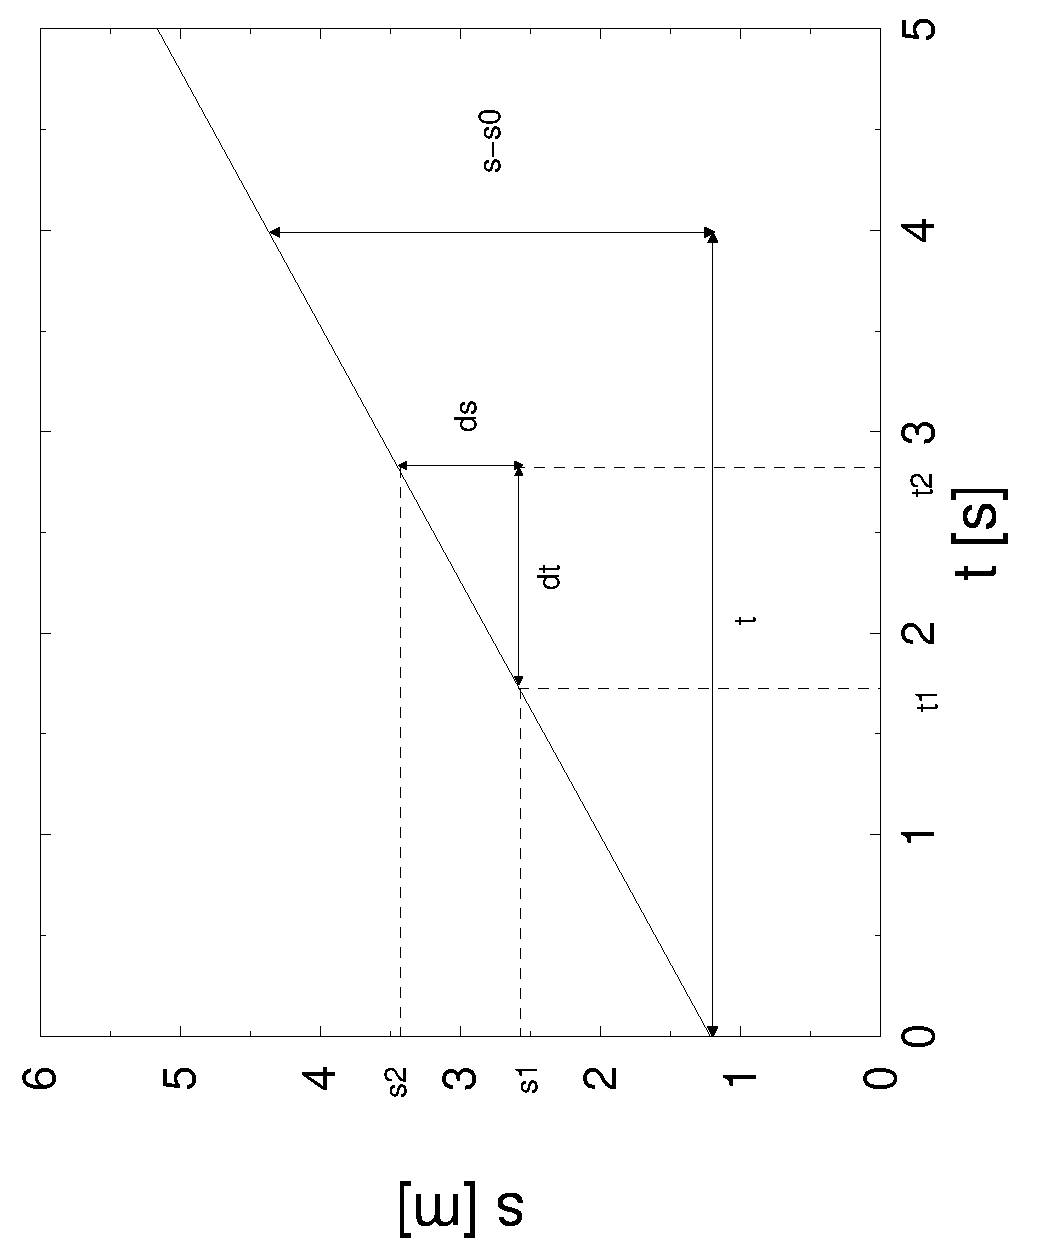
\includegraphics[angle=-90,width=\columnwidth]{pictures/stdreieck.eps}
  \caption{Steigungsdreiecke}
  \label{fig:linfkt2:stdreieck}
\end{figure}

Wenn wir eine Steigung im Gebirge berechnen, dividieren wir auch nicht die H\"ohe durch die Horizontaldistanz, sondern die H\"ohen\emph{differenz} durch die Horizontaldistanz. Wenn der Berg gleichm\"assig ansteigt, k\"onnen wir zur Berechnung der Steigung auch eine kurze Horizontaldistanz mitten auf dem Weg und die zugeh\"orige H\"ohendifferenz verwenden. Wir m\"ussen unsere Messungen also nicht unbedingt vom Startpunkt aus machen.

Genauso m\"ussen wir bei einer Bewegung mit konstanter Geschwindigkeit nicht unbedingt die seit dem Start zur\"uckgelegte Strecke durch die seither verstrichene Zeit dividieren. Wir k\"onnen ebensogut die Strecke bestimmen, die wir w\"ahrend einer kurzen Zeitspanne unterwegs zur\"ucklegen, und dann diese Strecke durch die zugeh\"orige Zeitspanne dividieren.

Beim H\"utchenexperiment arbeiten wir dann nicht direkt mit der Strecke, die wir auf dem Massstab ablesen, sondern mit einer Strecken\emph{differenz} $s_2-s_1$. Ebenso verwenden wir nicht direkt die Zeit auf der Messuhr, sondern eine Zeit\emph{differenz} $t_2-t_1$ (siehe kleines Steigungsdreieck in \ref{fig:linfkt2:stdreieck}):
\begin{displaymath}
  v = \frac{s_2-s_1}{t_2-t_1}
\end{displaymath}
In den vorangeganen Sections haben wir f\"ur Differenzen das Symbol $\Delta$ (grosses griechisches `Delta') eingef\"uhrt, welches wir vor das Gr\"ossensymbol setzen. Dementsprechend k\"onnen wir die Strecken- und Zeitdifferenzen so abk\"urzen (siehe \ref{fig:linfkt2:stdreieck}):\footnote{Ausgesprochen: `Delta s' und `Delta t'.}
\begin{eqnarray*}
  s_2-s_1 & = & \Delta s \\
  t_2-t_1 & = & \Delta t
\end{eqnarray*}
Dann k\"onnen wir die Definition der Geschwindigkeit so schreiben:
\begin{displaymath}
  v = \frac{\Delta s}{\Delta t}
\end{displaymath}
Wenn wir auf die Daten unserer Tabelle zur\"uckgreifen, k\"onnen wir die Geschwindigkeit \"uber die ganze Zeit von  $t=6\unit{s}$ hinweg berechnen:
\begin{displaymath}
  v= \frac{s - s_0}{t} = \frac{5.93\unit{m}-1.2\unit{m}}{6\unit{s}}=0.79\ufrac{m}{s}
\end{displaymath}
oder, indem wir die Streckendifferenz, die von der 1. bis zur 3. Sekunde zur\"uckgelegt wird, durch die entsprechende Zeitdifferenz dividieren:
\begin{displaymath}
  v= \frac{\Delta s}{\Delta t}=\frac{3.54\unit{m}-2.06\unit{m}}{3\unit{s}-1\unit{s}}=0.74\ufrac{m}{s}
\end{displaymath}
Die geringe Abweichung zwischen den beiden Geschwindigkeiten kommt durch die Ungenauigkeit der Tabellenwerte zustande. Wenn die Werte exakt auf einer Geraden liegen, ergeben sich auch exakt dieselben Geschwindigkeiten.

Eine Funktion, deren Graph eine Gerade ist, nennen wir linear. Wir haben es also immer noch mit linearen Funktionen zu tun. Beim H\"utchenbeispiel haben wir ja nur den Start verschoben bzw. die Gerade wurde im Diagramm aufw\"arts verschoben. Es kann also nichts v\"ollig Neues entstanden sein.

Im Folgenden werden wir \"ubrigens davon ausgehen, dass die Funktionen exakt linear sind, d.h. dass die Werte genau auf einer Geraden liegen.


\section{Die allgemeine Form der linearen Funktion}
\label{linfkt2:allgform}

Die allgemeine Form der linearen Funktionen sieht (mit $x$ und $y$ geschrieben) so aus:
\begin{displaymath}
  y=ax+b
\end{displaymath}
Das $x$ kommt bei linearen Funktionen nur in der 1. Potenz vor. Hingegen liegt keine lineare Funktion vor, wenn z.B. $x^2$ vorkommt oder das $x$ unter einer Wurzel erscheint ($\sqrt{x+5}$) oder in einem Exponenten ($3^x$). Ebenso wenig ist $y=\frac{1}{x}=x^{-1}$ eine lineare Funktion, denn dort steht das $x$ in der $-1.$ Potenz.

In der obigen Funktionsgleichung ist $a$ nach wie vor die Steigung der Geraden, die sich als Graph ergibt. Diese Steigung erhalten wir, wenn wir eine \quasi{H\"ohendifferenz} $\Delta y=y_2-y_1$ durch die zugeh\"orige \quasi{Horizontaldistanz} $\Delta x = x_2-x_1$ dividieren\footnote{Die Begriffe \quasi{H\"ohendifferenz} und \quasi{Horizontaldistanz} verwenden wir hier nur symbolisch. Das $x$ kann ja z.B. f\"ur die Zeit stehen. Das $y$ kann z.B. die zur\"uckgelegte Strecke sein oder die Temperatur zu einem bestimmten Zeitpunkt. $\Delta x$ und $\Delta y$ sind dann entsprechende Differenzen.}:
\begin{displaymath}
  a=\frac{\Delta y}{\Delta x} = \frac{y_2 - y_1}{x_2 - x_1}
\end{displaymath}

Gegen\"uber den Funktionen $y=ax$ wird nun zu jedem $y$ ein fester Wert $b$ dazugez\"ahlt. Deshalb geht die Gerade nicht mehr durch den Ursprung, sondern ist um $b$ nach oben verschoben.

Das kann man am besten auf der $y$-Achse ablesen. Die Gerade passiert diese eben nicht mehr auf der H\"ohe Null, sondern auf der H\"ohe $b$ (siehe \ref{fig:linfkt2:axplusb}). Deshalb nennen wir $b$ den $y$-\emph{Achsenabschnitt}.

\begin{figure}[b!]
  \centering
  \psfrag{dx}{$\Delta x$} \psfrag{dy}{$\Delta y$} \psfrag{x1}{$x_1$} \psfrag{x2}{$x_2$} \psfrag{y1}{$y_1$} \psfrag{y2}{$y_2$} \psfrag{a2}{$a\cdot 2$} \psfrag{a}{$a$} \psfrag{b}{$b$}
  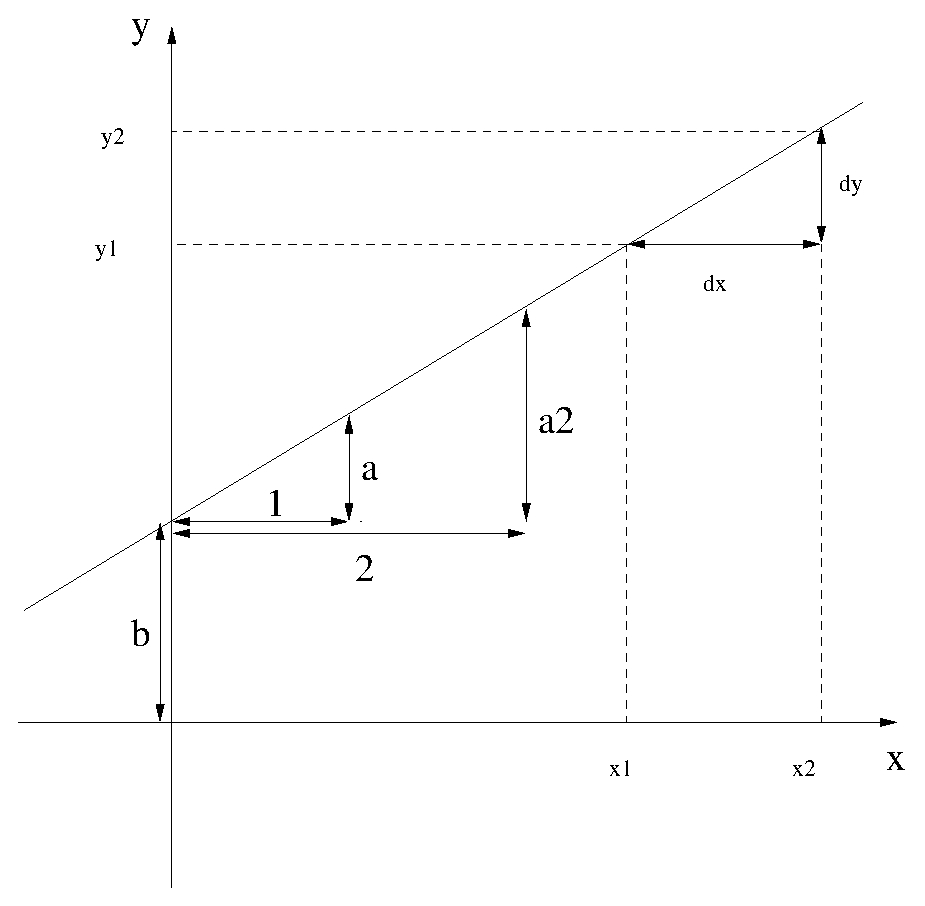
\includegraphics[width=0.8\columnwidth]{pictures/axplusb.eps}
  \caption{Eine lineare Funktion der Form $y=ax+b$.}
  \label{fig:linfkt2:axplusb}
\end{figure}

Das k\"onnen wir auch in der Funktionsgleichung nachvollziehen. Die $y$-Achse umfasst n\"amlich alle Punkte, f\"ur die $x=0$ ist. Um den Schnittpunkt der Geraden mit der $y$-Achse zu erhalten, m\"ussen wir also $x=0$ setzen. Dann ergibt sich $y=a\cdot 0 + b = b$. Das heisst: die Gerade schneidet die $y$-Achse bei $y=b$, wie wir gesagt haben.

Wir haben nun also dasselbe wie im vorangegangenen Kapitel, aber um $b$ nach oben verschoben. (Wenn $b=0$ ist, liegt allerdings wieder der Spezialfall aus der Section von vorhin vor\,\ldots.)

\section{Wie zeichnet man eine gegebene lineare Funktion?}
\label{linfkt2:zeichnen}

Wenn wir z.B. die Gerade
\begin{displaymath}
  y = 2x + 3
\end{displaymath}
zeichnen wollen, k\"onnten wir zuerst eine Tabelle machen. Wir k\"onnten f\"ur verschiedene $x$ mit Hilfe der Funktionsgleichung das zugeh\"orige $y$ berechnen. Dadurch erg\"abe sich \ref{tab:linfkt2:2xplus3}.

\begin{table}[b!]
\centering
\begin{tabular}{|c|c|}
\hline
$x$ & $y$ ($=2x+3$) \\ \hline\hline
-5 & -7 \\ \hline
-4 & -5 \\ \hline
-3 & -3 \\ \hline
-2 & -1 \\ \hline
-1 & 1 \\ \hline
0 & 3 \\ \hline
1 & 5 \\ \hline
2 & 7 \\ \hline
3 & 9 \\ \hline
4 & 11 \\ \hline
5 & 13 \\ \hline
\end{tabular}
\caption{Wertetabelle der Funktion $y=2x+3$}
\label{tab:linfkt2:2xplus3}
\end{table}

Dann k\"onnen wir die Punkte in ein Koordinatensystem eintragen und sie verbinden. So erg\"abe sich \ref{fig:linfkt2:2xplus3}.

\begin{figure}[b!]
  \centering
  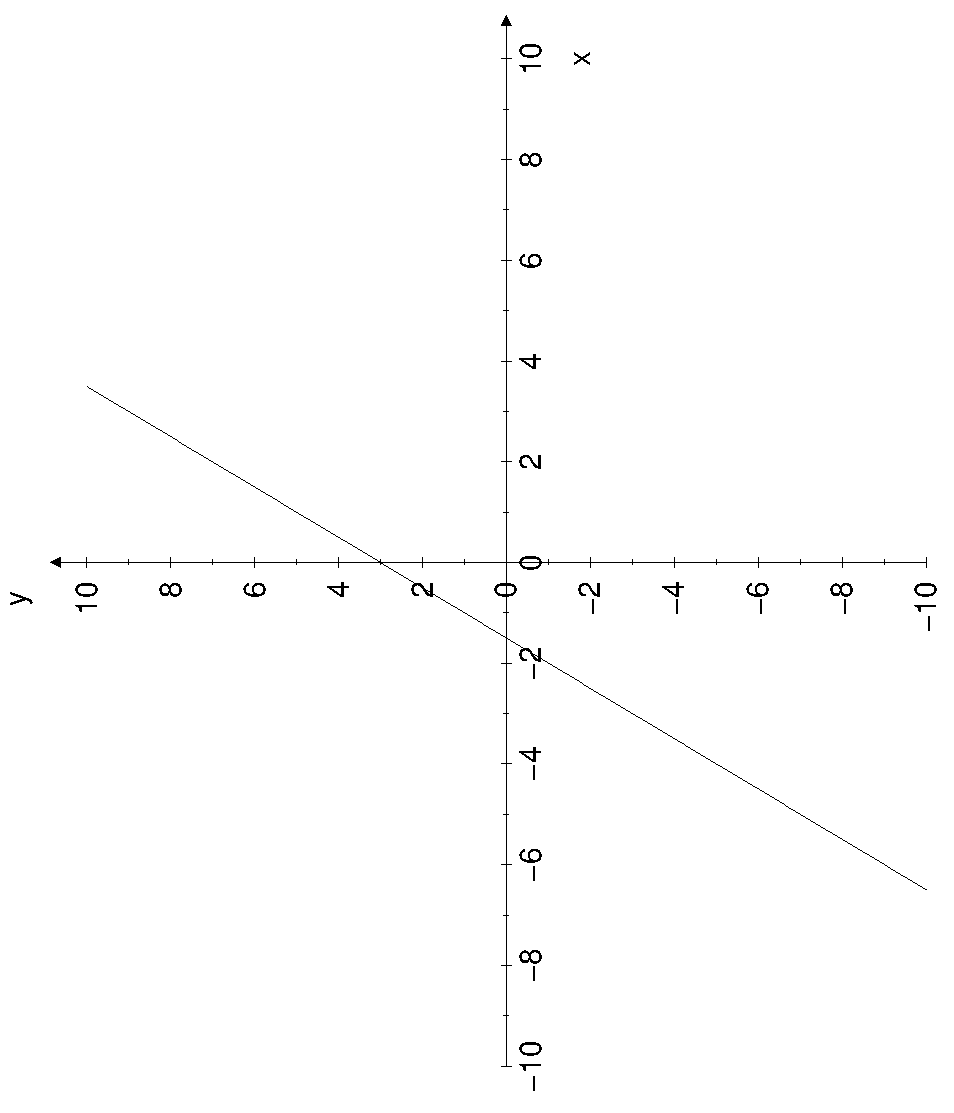
\includegraphics[angle=-90,width=\columnwidth]{pictures/2xplus3.eps}
  \caption{Der Graph der Funktion $y=2x+3$}
  \label{fig:linfkt2:2xplus3}
\end{figure}

Allerdings ist das zu kompliziert. Es w\"urde reichen, nur zwei Punkte zu berechnen, die nicht zu nahe bei einander liegen, damit's nicht zu ungenau wird. Weil wir wissen, dass es sich um eine lineare Funktion handelt, k\"onnen wir dann die Gerade durch die beiden Punkte hindurch ziehen.

Doch es geht noch direkter: Direkt aus der Gleichung k\"onnen wir n\"amlich die Steigung $a=2$ und den $y$-Achsenabschnitt $b=3$ ablesen. Wir wissen, dass die Gerade die $y$-Achse auf der H\"ohe $b=3$ passiert. Diesen Punkt auf der $y$-Achse markieren wir. Davon ausgehend zeichnen wir die Gerade mit Hilfe der Steigung, so wie wir es bei Proportionalit\"aten vom Ursprung ausgehend getan haben: Die H\"ohendifferenz ist immer doppelt so gross wie die Horizonaldistanz. Auch so ergibt sich der Graph in \ref{fig:linfkt2:2xplus3}.

Das Vorgehen ist also generell wie folgt: Wenn die Funktionsgleichung gegeben ist, gehen wir einfach auf der $y$-Achse um $b$ nach oben. Dort passiert ja die Gerade die $y$-Achse. Von dort aus zeichnen wir sie mit der entsprechenden Steigung: die H\"ohendifferenz ist immer $a$-mal so gross wie die Horizontaldistanz. (siehe \ref{fig:linfkt2:axplusb}).


\section{Steigung und ein Punkt gegeben}
\label{linfkt2:a+pktgeg}

Die konstante Geschwindigkeit eines Fahrzeugs sei $v=15\ufrac{m}{s}$. Ausserdem wissen wir, dass es nach 6\unit{s} bei 140\unit{m} angelangt ist (was wir am Messtreifen entlang unserer Teststrecke ablesen). Wie sieht dann die Funktionsgleichung f\"ur die ganze Bewegung aus?

\begin{figure}[b!]
  \centering
  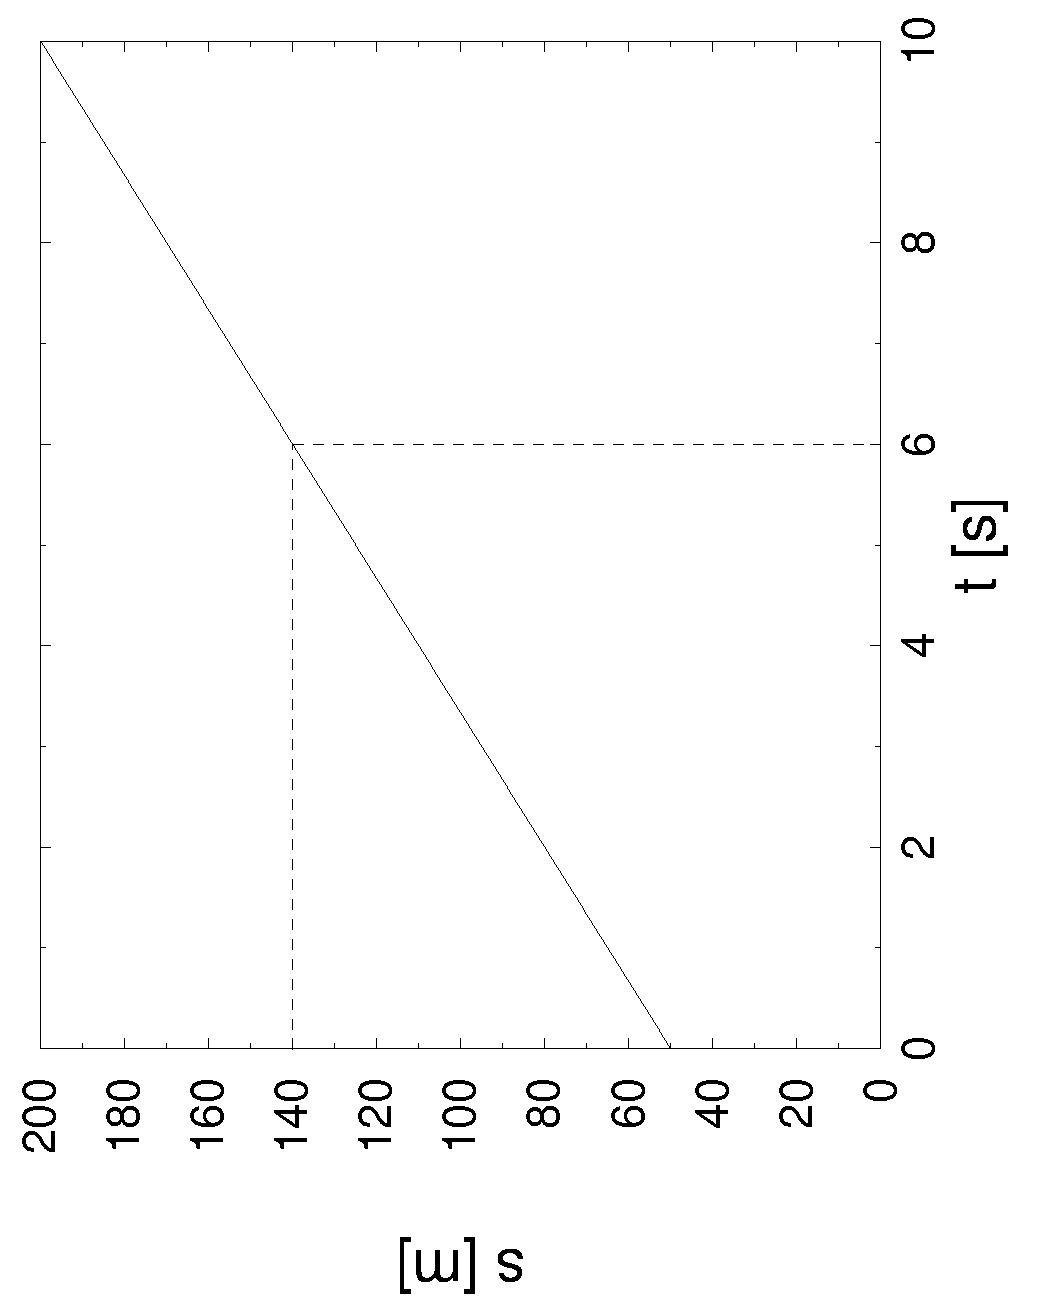
\includegraphics[angle=-90,width=\columnwidth]{pictures/fahrzeug.eps}
  \caption{Die Bewegung eines Fahrzeugs mit der Geschwindigkeit $v=15\ufrac{m}{s}$, das nach 6\unit{s} bei 140\unit{m} angelangt ist.}
  \label{fig:linfkt2:fahrzeug}
\end{figure}

Wir wissen nicht, ob beim Start der Uhr ($t=0$) das Fahrzeug bei $s=0$ war (d.h. ob $s_0=0$ ist). Deshalb k\"onnen wir nicht einfach von der Formel $s=vt$ ausgehen (wie in Kapitel 10), sondern m\"ussen auf die allgemeine Form der linearen Funktionsgleichung zur\"uckgreifen:
\begin{displaymath}
  s = vt + s_0
\end{displaymath}
Wenn wir die Geschwindigkeit, die wir ja kennen, einsetzen, ergibt sich:
\begin{displaymath}
  s = 15\ufrac{m}{s}\,t + s_0
\end{displaymath}
Wir wissen, dass zur Zeit $t=6\unit{s}$ die Strecke $s=140\unit{m}$ ist. F\"ur diese Werte muss die Funktionsgleichung gelten, denn sie liefert ja zu jedem Zeitpunkt $t$ die zugeh\"orige Strecke $s$, bei der sich das Fahrzeug dann befindet. Wir k\"onnen also diese Werte f\"ur $s$ und $t$ einsetzen, um $s_0$ auszurechnen:
\begin{eqnarray*}
  140\unit{m} & = & 15\ufrac{m}{s} \cdot 6\unit{s} + s_0 \\
  s_0 & = & 140\unit{m}-90\unit{m} = 50\unit{m}
\end{eqnarray*}
Demnach ist das Fahrzeug zur Zeit $t=0$ bei $s_0=50\unit{m}$ gestartet. Die Funktionsgleichung lautet somit:
\begin{displaymath}
  s = 15\ufrac{m}{s}t + 50\unit{m}
\end{displaymath}
Der Graph ist in \ref{fig:linfkt2:fahrzeug} dargestellt.

In einem rein mathematischen Beispiel sieht das so aus: Die Steigung der Geraden sei gegeben: $a=2.5$. Ausserdem wissen wir, dass die Gerade durch den Punkt $(3|5)$ geht. Zun\"achst setzen wir die gegebene Steigung in die allgemeine Funktionsgleichung ein:
\begin{displaymath}
  y = 2.5x + b
\end{displaymath}
Diese Gleichung gilt f\"ur die ganze Gerade, insbesondere f\"ur den Punkt $(3|5)$, der gegeben ist. F\"ur $x=3$ muss sie also $y=5$ liefern:
\begin{displaymath}
  5 = 2.5 \cdot 3 + b
\end{displaymath}
Daraus erhalten wir problemlos $b$:
\begin{displaymath}
  b = 5 - 2.5 \cdot 3 = -2.5
\end{displaymath}
Die Gerade passiert also die $y$-Achse bei $-2.5$. Die Funktionsgleichung ist somit:
\begin{displaymath}
  y = 2.5x - 2.5
\end{displaymath}
Der Graph ist in \ref{fig:linfkt2:a+pktgeg} dargestellt.

\begin{figure}[b!]
  \centering
  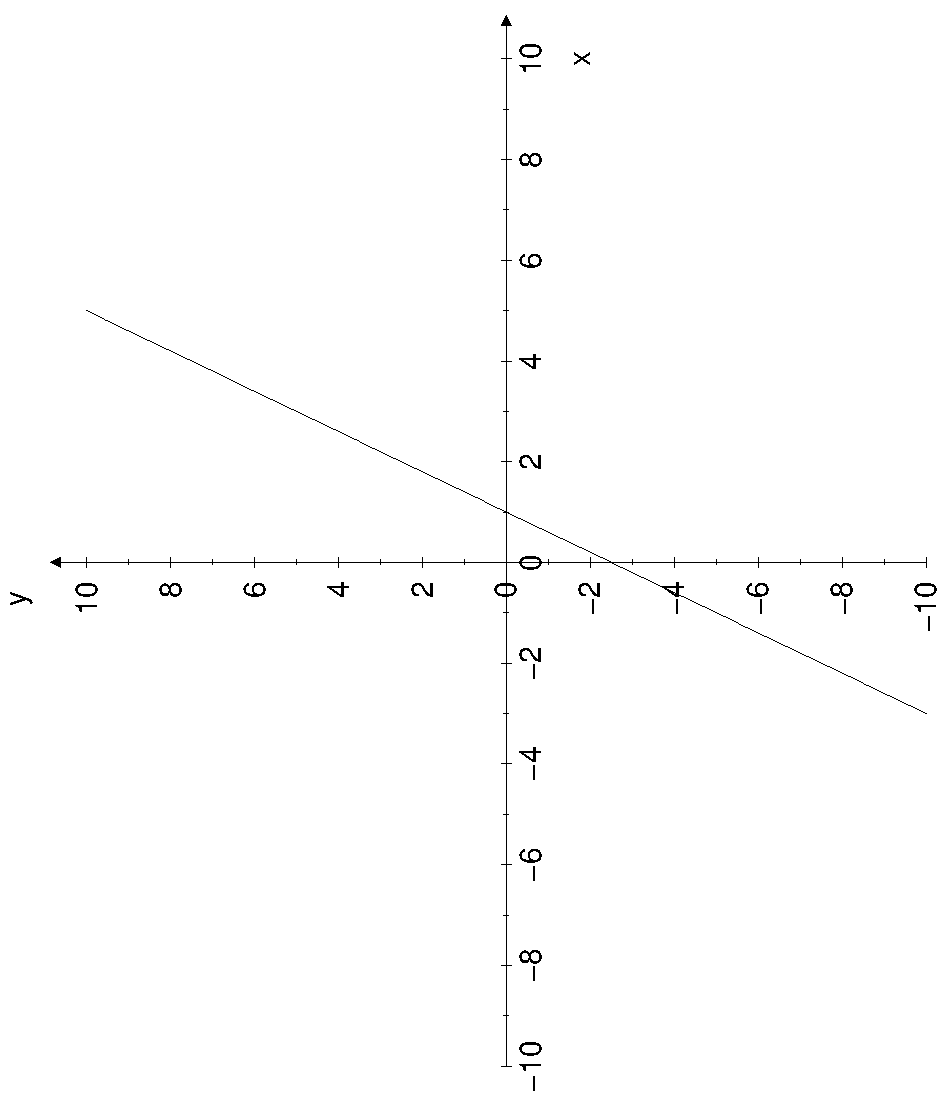
\includegraphics[angle=-90,width=\linewidth]{pictures/a+pktgeg.eps}
  \caption{Graph der Funktion $y=2.5x-2.5$}
  \label{fig:linfkt2:a+pktgeg}
\end{figure}

\section{Zwei Punkte gegeben}
\label{linfkt2:2pktgeg}

Eine Gerade ist durch zwei Punkte eindeutig bestimmt. Wir k\"onnen also zwei Punkte vorgeben und dann erwarten, dass man die Funktionsgleichung der zugeh\"origen linearen Funktion bestimmen kann. Z.B. seien die Punkte $(2|5)$ und $(5|6.5)$ gegeben.

Als erstes bestimmen wir in einem solchen Fall die Steigung $a$. Dann k\"onnen wir n\"amlich vorgehen wie im vorangegangenen Abschnitt, weil $a$ bekannt ist und (mindestens) ein weiterer Punkt.

Wie finden wir $a$? Erinnern wir uns daran, dass wir die Steigung mit Hilfe von Differenzen $\Delta x$ und $\Delta y$ berechnen k\"onnen:
\begin{displaymath}
  a=\frac{\Delta y}{\Delta x} = \frac{y_2 - y_1}{x_2 - x_1}
\end{displaymath}
Dabei stehen $x_1$, $y_1$, $x_2$ und $y_2$ f\"ur die Koordinaten zweier Punkte: $(x_1|y_1)$ und $(x_2|y_2)$ (siehe \ref{fig:linfkt2:axplusb}). Genau das ist gegeben, n\"amlich die Koordinaten der Punkte $(2|5)$ und $(5|6.5)$. Damit ergibt sich:
\begin{displaymath}
  a = \frac{6.5 - 5}{5-2} = \frac{1}{2}
\end{displaymath}
Die Funktionsgleichung sieht damit so aus:
\begin{displaymath}
  y = \frac{1}{2}x + b
\end{displaymath}
Diese Gleichung muss nat\"urlich auch f\"ur die beiden gegebenen Punkte gelten. Wenn wir einen davon --- z.B. $(2|5)$ --- einsetzen, finden wir $b$:
\begin{eqnarray*}
  5 & = & \frac{1}{2} \cdot 2 + b \\
  b & = & 5 - 1 = 4
\end{eqnarray*}
Wenn wir den anderen Punkt $(5|6.5)$ einsetzen, kommen wir zum selben Resultat:
\begin{eqnarray*}
  6.5 & = & \frac{1}{2} \cdot 5 + b \\
  b & = & 6.5 - 2.5 = 4
\end{eqnarray*}
Das muss nat\"urlich so sein. Es reicht also, wenn wir einen Punkt einsetzen, um $b$ zu finden. Den zweiten setzen wir nur ein, wenn wir das Resultat kontrollieren m\"ochten.

Nun haben wir die Funktionsgleichung gefunden:
\begin{displaymath}
  y=\frac{1}{2}x + 4
\end{displaymath}
Der Graph ist in \ref{fig:linfkt2:2pktgeg} dargestellt.

\begin{figure}[t!]
  \centering
  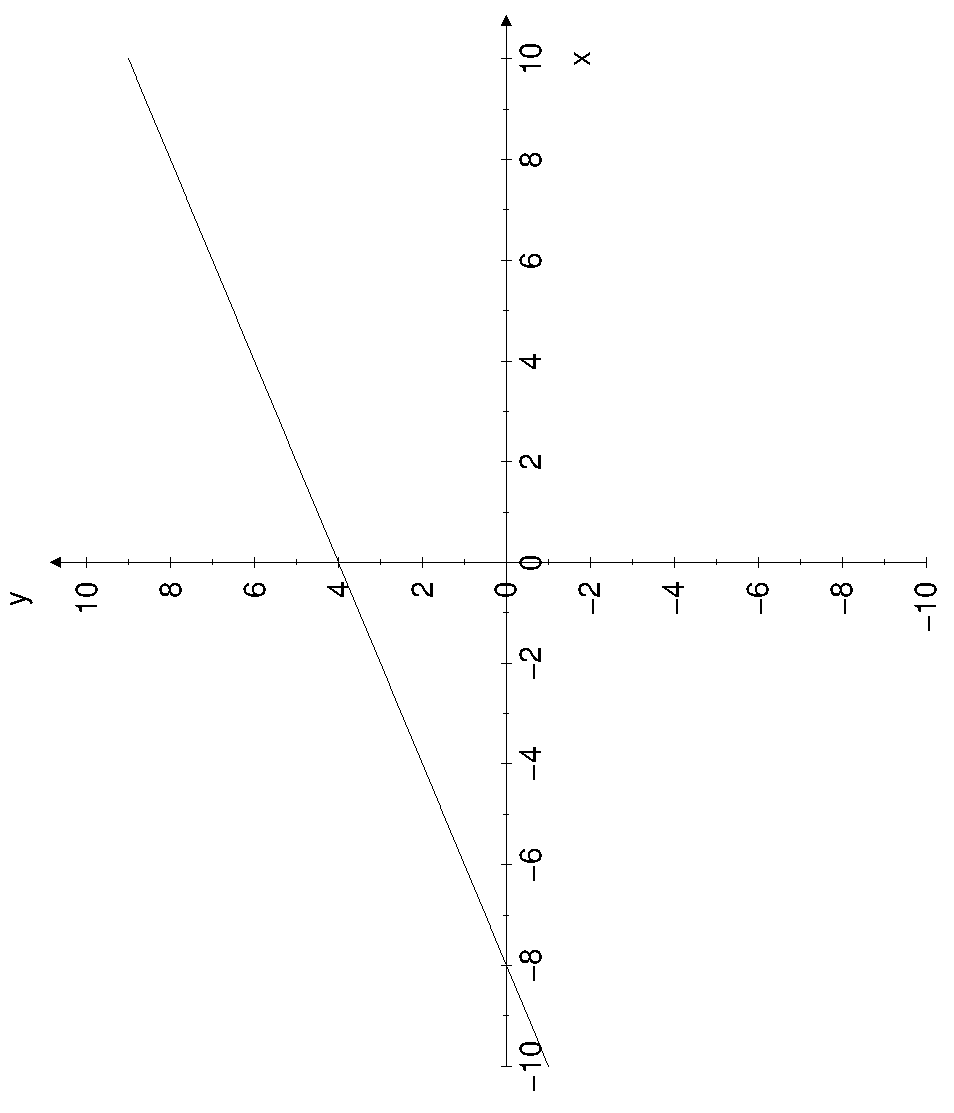
\includegraphics[angle=-90,width=\linewidth]{pictures/2pktgeg.eps}
  \caption{Der Graph der Funktion $y=\frac{1}{2}x+4$}
  \label{fig:linfkt2:2pktgeg}
\end{figure}




%\section*{Lernziele \thesection}
{\settowidth{\labelwidth}{\labelitemi}
\setlength{\leftmargini}{\labelwidth} \addtolength{\leftmargini}{\labelsep}
%Sie k\"onnen\dots
%\begin{itemize}
%\item \dots die allgemeine Form ($y=ax+b$) einer linearen Funktion angeben und erkl\"aren, was $a$ und $b$ bedeuten
%\item \dots lineare von nicht-linearen Funktionen unterscheiden
%\item \dots jede lineare Funktion (der Form $y=ax+b$) effizient zeichnen
%\item \dots die Funktionsgleichung einer linearen Funktion bestimmen, \dots
%  \begin{itemize}
%  \item \dots wenn die Steigung und ein Punkt gegeben sind
%  \item \dots wenn zwei Punkte gegeben sind
%  \end{itemize}
%\item \dots die Funktionsgleichung einer linearen Funktion bestimmen, wenn deren Graph gegeben ist
%\item \dots den Schnittpunkt einer Geraden mit der $x$- bzw. $y$-Achse bestimmen
%\end{itemize}}


\section*{Aufgaben}
{\settowidth{\labelwidth}{19.19}
\setlength{\leftmargini}{\labelwidth} \addtolength{\leftmargini}{\labelsep}
\renewcommand{\labelenumi}{\thesection.\arabic{enumi}}
\begin{enumerate}
\item Welche der folgenden Funktionen sind linear?
  \begin{enumerate}
  \item $\displaystyle y=\frac{1}{2x-1}$
  \item $\displaystyle y=x+3\sqrt{x}-2$
  \item \label{aufg:linfkt2:linear1} $\displaystyle y=\frac{6-2x}{5}$
  \item $\displaystyle y=2^x-x$
  \item $\displaystyle y=\frac{x-a}{x-b}$
  \item $\displaystyle y=a^2x-a-\frac{1}{x}$
  \item \label{aufg:linfkt2:linear2} $\displaystyle y=a^2x-a-1$
  \item \label{aufg:linfkt2:linear3} $\displaystyle y=xb-2x+3$
  \item \label{aufg:linfkt2:linear4} $\displaystyle y=\frac{a^2-ax}{5b}$
  \item \label{aufg:linfkt2:linear5} $\displaystyle y=2\pi x + b$
  \item \label{aufg:linfkt2:linear6} $\displaystyle y=(x-n)^2-x^2$
  \end{enumerate}
\item Wie lautet die Funktionsgleichung zur Geraden, deren Steigung 4 ist und welche die $y$-Achse bei $y=-5$ passiert?

\item Wie lauten die Antworten zu Aufgabe \ref{linfkt1}.\ref{aufg:linfkt1:stoff}, wenn f\"ur das Zurechtschneiden und den Versand unabh\"angig von der Stoffmenge eine Pauschale von Fr.~30.- berechnet wird?

\item Wie lauten die Antworten zu den Aufgaben \ref{linfkt1}.\ref{aufg:linfkt1:federgraph}, \ref{linfkt1}.\ref{aufg:linfkt1:federgl}, \ref{linfkt1}.\ref{aufg:linfkt1:federbsp}, wenn \"uberall anstelle der Verl\"angerung von der Gesamtl\"ange der Feder die Rede ist?

\newcounter{uaufg}
\setcounter{uaufg}{0}
\item Zeichnen Sie die Graphen folgender Funktionen:
  \begin{enumerate}
  \item $\displaystyle y=3x+4$
  \item $\displaystyle y=3x-4$
  \item $\displaystyle y=-3x+4$
  \item $\displaystyle y=1.5x-3$
  \item $\displaystyle y=-1.5x+3$
  \item $\displaystyle y=-0.5x-2$
  \item $\displaystyle y=-\frac{2}{3}x+1$
  \item $\displaystyle y=-2x$
  \item $\displaystyle y=2$
  \item $\displaystyle y=\frac{2}{5}x+1$
  \item \label{aufg:linfkt2:zeichnen1} $\displaystyle -4x+2y+3=0$
  \item \label{aufg:linfkt2:zeichnen2} $\displaystyle x-y-1=0$
  \item \label{aufg:linfkt2:zeichnen3} $\displaystyle 2x=3y$
  \end{enumerate}


\item Wie lauten die Funktionsgleichungen, welche die Geraden in \ref{fig:linfkt2:ablesen} als Graphen haben?

\begin{figure}[b!]
  \centering
  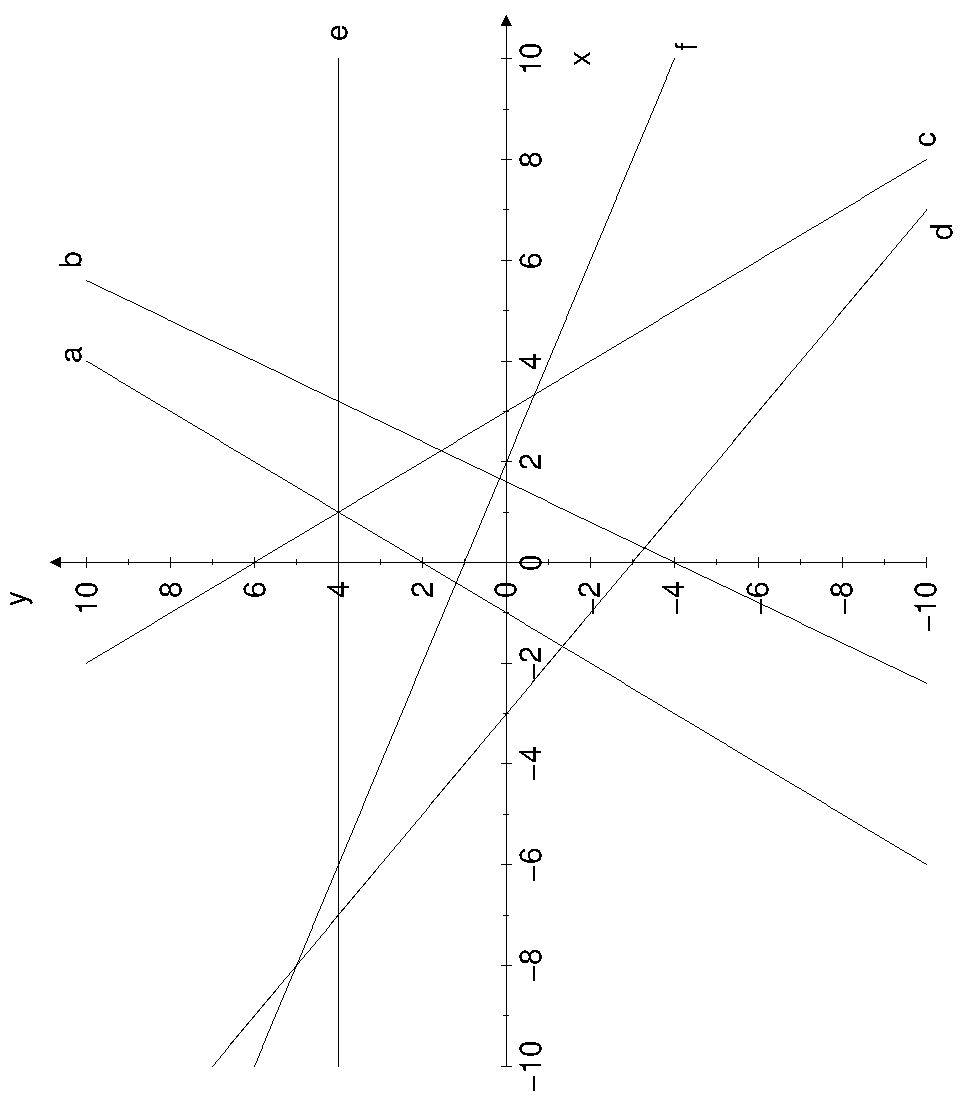
\includegraphics[angle=-90,width=\linewidth]{pictures/ablesen.eps}
  \caption{Gesucht sind die Funktionsgleichungen, die zu diesen Geraden geh\"oren.}
  \label{fig:linfkt2:ablesen}
\end{figure}


\item Geben Sie zur jeweiligen Wertetabelle die Funktionsgleichung an:
  \begin{enumerate}
  \item 
    \begin{tabular}{|c|c|} 
      \hline 
      x & y \\ \hline\hline
      0 & 2.5 \\ \hline
      1 & 4.5 \\ \hline
    \end{tabular}
  \item 
    \begin{tabular}{|c|c|} 
      \hline 
      x & y \\ \hline\hline
      0 & -1 \\ \hline
      1 & -2 \\ \hline
    \end{tabular}
  \item 
    \begin{tabular}{|c|c|} 
      \hline 
      x & y \\ \hline\hline
      0 & 2.6 \\ \hline
      1 & -0.8 \\ \hline
    \end{tabular}
  \end{enumerate}

\item Welche der Punkte 

$P_1(1|1.6)$

$P_2(-1|-1.6)$

$P_3(-2.5|-0.2)$

$P_4(1.6|-1.84)$

\noindent
liegen auf der Geraden $y=-0.4x-1.2$?

\item Finden Sie die Funktionsgleichungen der linearen Funktionen, von denen jeweils die Steigung $a$ und ein Punkt gegeben sind, und zeichnen Sie ihre Graphen:
  \begin{enumerate}
  \item $a=2$, $(-1|3)$
  \item $a=-2$, $(2.5|1)$
  \item $a=-1$, $(3|-2.5)$
  \item $a=\frac{3}{2}$, $(0|-2)$
  \item $a=-\frac{1}{2}$, $(-4|0)$
  \item $a=\frac{3}{5}$, $(\frac{2}{3}|-\frac{1}{3})$
  \end{enumerate}

\item Finden Sie die Funktionsgleichungen der linearen Funktionen, von denen jeweils zwei Punkte gegeben sind, und zeichnen Sie ihre Graphen:
  \begin{enumerate}
  \item $(2|4)$, $(6|12)$
  \item $(-2|-3)$, $(1|-1.5)$
  \item $(3|1)$, $(1|-1)$
  \item $(-4|-2)$, $(0|-4)$
  \item $(3|-1)$, $(1|3)$
  \item $(-2.5|3)$, $(1.5|3)$
  \item $(3|0)$, $(0|4)$
  \end{enumerate}

\item Der $y$-Achsenabschnitt einer linearen Funktion sei $b=-3$. Ausserdem ist der Punkt $(3|1)$ gegeben. Wie lautet Funktionsgleichung? Zeichnen Sie die Gerade.

\item Bestimmen Sie die Koordinaten des Schnittpunkts der Geraden mit der $y$-Achse:
  \begin{enumerate}
  \item $y=2x-3$
  \item $y=3x+4$
  \item $y=-x+1$
  \item $y=-2x-2$
  \item $y=-5+x$
  \item $y=4x$
  \item $y=-\frac{1}{2}x+8$
  \item $y=\frac{3}{4}x-4$
  \item $y=1-0.5x$
  \item $y=6-x$
  \item $y=\frac{x}{5}$
  \item $y=9-\frac{2}{3}x$
  \end{enumerate}

\item Bestimmen Sie den Schnittpunkt der Geraden mit der $x$-Achse:
  \begin{enumerate}
  \item $y=3x+3$
  \item $y=2x-1$
  \item $y=5x-2.5$
  \item $y=6x-3$
  \item $12=\frac{1}{4}x-y$
  \item $x=\frac{3}{5}-y$
  \item $y-\frac{2}{7}=-4x$
  \item $3y-9x=6$
  \item $3y-12=x$
  \item $x-2y=6$
  \item $2x-6y+3=0$
  \item $x+3y-3=0$
  \end{enumerate}

\item Wie lautet die Funktionsgleichung der Geraden durch den Punkt $(3|-1)$, die parallel zur Geraden $y=-2x+1$ verl\"auft?


\item Zur Zeit $t=0$ startet ein Zug 120\unit{km} von uns entfernt und bewegt sich mit 90\ufrac{km}{h} auf uns zu. Wie lautet die Funktionsgleichung f\"ur die Distanz im Lauf der Zeit? Zeichnen Sie den Graphen dieser Funktion.

\item Aus einem 3\unit{m} tiefen Wasserbecken wird das Wasser abgelassen, wobei der Wasserspiegel st\"undlich um 35\unit{cm} sinkt. Wie lautet die Funktionsgleichung f\"ur die H\"ohe des Wasserspiegels im Lauf der Zeit?

\end{enumerate}}


\section*{L\"osungen}
{\settowidth{\labelwidth}{L19.19}
\setlength{\leftmargini}{\labelwidth} \addtolength{\leftmargini}{\labelsep}
\renewcommand{\labelenumi}{L\thesection.\arabic{enumi}}
\begin{enumerate}

\item Linear sind \ref{aufg:linfkt2:linear1}, \ref{aufg:linfkt2:linear2}, \ref{aufg:linfkt2:linear3}, \ref{aufg:linfkt2:linear4}, \ref{aufg:linfkt2:linear5} und \ref{aufg:linfkt2:linear6}.
\item $a=4$, $b=-5$: $\result{y=4x-5}$

\item $l$: L\"ange, $p$: Preis
  \begin{displaymath}
    \result{p=12.5\ufrac{Fr.}{m} \cdot l + 30\unit{Fr.}}
  \end{displaymath}

\begin{center}
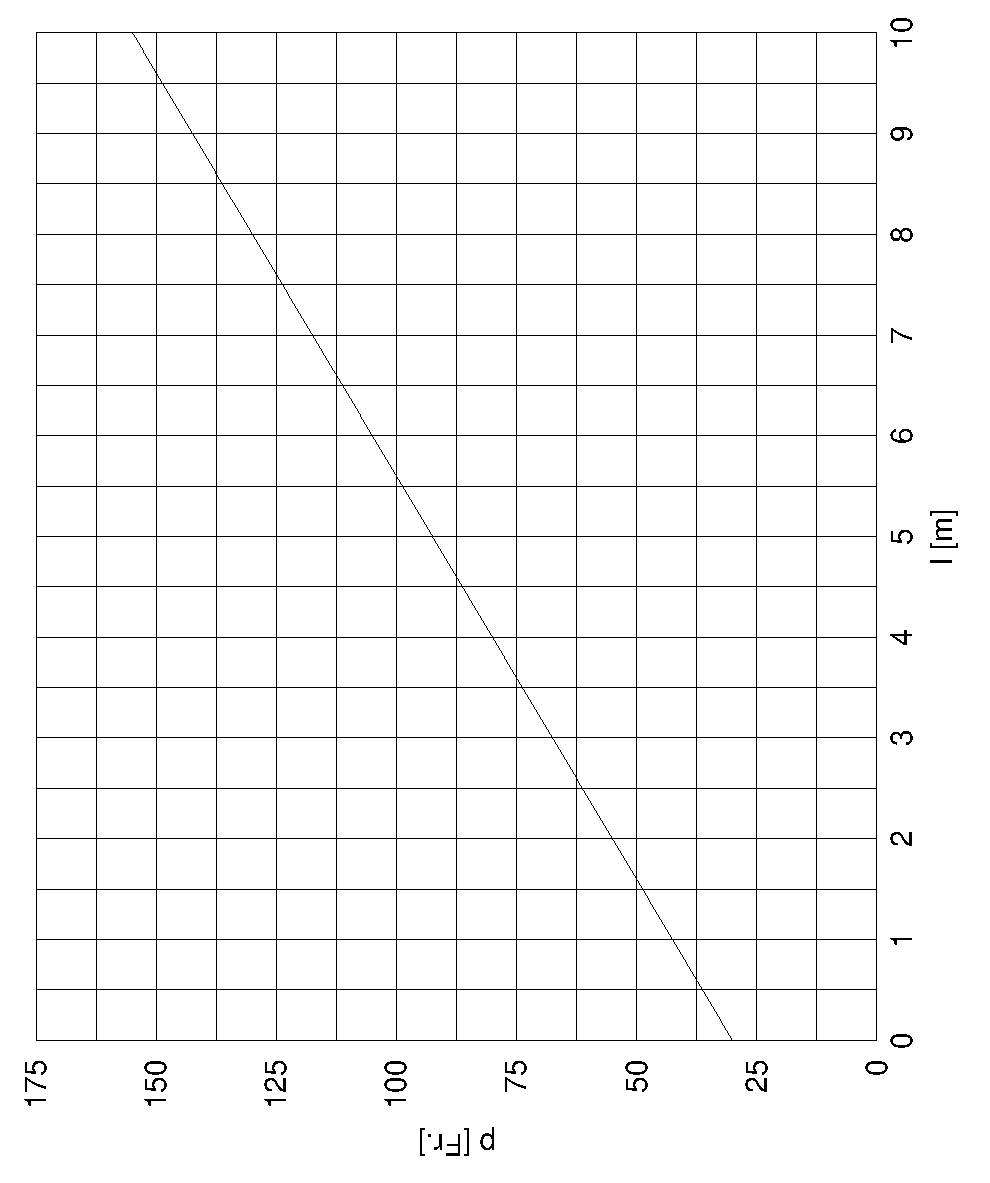
\includegraphics[angle=-90,width=0.8\linewidth]{pictures/stoffb.eps}
\end{center}

4\unit{m}: $\result{80\unit{Fr.}}$; 2.5\unit{m}: $\result{61.25\unit{Fr.}}$; 7\unit{m}: $\result{117.50\unit{Fr.}}$; 5.4\unit{m}: $\result{97.50\unit{Fr.}}$


\item $l$ steht nun f\"ur die totale L\"ange.
  \begin{enumerate}
  \item Tabelle:
    \begin{center}
      \begin{tabular}{|c|c|}
        \hline
        $m$\,[kg] & $l$\,[cm] \\ \hline\hline
        0 & 6 \\ \hline
        2 & 7.2 \\ \hline
        4 & 8.5 \\ \hline
        6 & 9.7 \\ \hline
        8 & 10.7 \\ \hline
        10 & 12 \\ \hline
      \end{tabular}
    \end{center}
    
    \begin{center}
      \psfrag{dl [cm]}[][][0.8]{$l$ [cm]}
      \includegraphics[width=\linewidth]{pictures/flfeder+.eps}
    \end{center}
    
    \addtocounter{enumii}{1}
    
\item Zu allen L\"angenwerten kommt einfach $l_0=6\unit{cm}$ dazu:
\begin{eqnarray*}
  l & = & \Delta l+l_0 \\
  l & = & \frac{1}{D}F+l_0 \\
  l & = & \frac{1}{17}\ufrac{cm}{N}\cdot F+6\unit{cm}
\end{eqnarray*}

  \item $F=72\unit{N}$: $\Delta l=10.2\unit{cm}$
  \end{enumerate}


\item 

    \begin{center}
\definecolor{ccqqqq}{rgb}{0.8,0,0}
\definecolor{qqwuqq}{rgb}{0,0.39215686274509803,0}
\scalebox{0.618}{
\begin{tikzpicture}[line cap=round,line join=round,>=triangle 45,x=1cm,y=1cm]
\begin{axis}[
x=1cm,y=1cm,
axis lines=middle,
ymajorgrids=true,
xmajorgrids=true,
xmin=-8.0,
xmax=9.2,
ymin=-4.8,
ymax=6.9,
xtick={-7,-6,...,9},
ytick={-5,-4,...,6},]
\clip(-8.3,-5.3) rectangle (9.6,6.9);
\draw[line width=2pt,color=qqwuqq,smooth,samples=100,domain=-8.16:9.40] plot(\x,{3*(\x)+4});
\draw[line width=2pt,color=ccqqqq,smooth,samples=100,domain=-8.16:9.40] plot(\x,{(3)*(\x)-4});
\draw[line width=2pt,color=ccqqqq,smooth,samples=100,domain=-8.16:9.40] plot(\x,{(-3)*(\x)+4});
\draw[line width=2pt,color=ccqqqq,smooth,samples=100,domain=-8.16:9.40] plot(\x,{(1.5)*(\x)-3});
\draw[line width=2pt,color=ccqqqq,smooth,samples=100,domain=-8.16:9.40] plot(\x,{(-0.5)*(\x)-2});
\draw[line width=2pt,color=ccqqqq,smooth,samples=100,domain=-8.16:9.40] plot(\x,{(3)*(\x)-4});
\begin{scriptsize}
%\draw[color=qqwuqq] (-6.72,-3.73) node {$f$};
%\draw[color=ccqqqq] (-4.22,5.79) node {$g$};
\draw[color=black] (8.8,0.3) node {$x$};
\draw[color=black] (-0.4,6.5) node {$y$};
\end{scriptsize}
\end{axis}
\end{tikzpicture}
}
\end{center}

F\"ur die drei letzten Unteraufgaben ergeben sich folgende Funktionsgleichungen in der Standard-Form:
  \begin{eqnarray*}
    \ref{linfkt2}.\ref{aufg:linfkt2:zeichnen1}: \quad y & = & 2x-\frac{3}{2} \\
    \ref{linfkt2}.\ref{aufg:linfkt2:zeichnen2}:  \quad y & = & x-1 \\
    \ref{linfkt2}.\ref{aufg:linfkt2:zeichnen3}: \quad y & = & \frac{2}{3}x
  \end{eqnarray*}

    \begin{center}
\definecolor{ccqqqq}{rgb}{0.8,0,0}
\definecolor{qqwuqq}{rgb}{0,0.39215686274509803,0}
\scalebox{0.618}{
\begin{tikzpicture}[line cap=round,line join=round,>=triangle 45,x=1cm,y=1cm]
\begin{axis}[
x=1cm,y=1cm,
axis lines=middle,
ymajorgrids=true,
xmajorgrids=true,
xmin=-8.0,
xmax=9.2,
ymin=-4.8,
ymax=6.9,
xtick={-7,-6,...,9},
ytick={-5,-4,...,6},]
\clip(-8.3,-5.3) rectangle (9.6,6.9);
\draw[line width=2pt,color=qqwuqq,smooth,samples=100,domain=-8.16:9.40] plot(\x,{-2/3*(\x)+1});
\draw[line width=2pt,color=ccqqqq,smooth,samples=100,domain=-8.16:9.40] plot(\x,{(-2)*(\x)});
\draw[line width=2pt,color=ccqqqq,smooth,samples=100,domain=-8.16:9.40] plot(\x,{2});
\draw[line width=2pt,color=ccqqqq,smooth,samples=100,domain=-8.16:9.40] plot(\x,{(2/5)*(\x)+1});
\draw[line width=2pt,color=ccqqqq,smooth,samples=100,domain=-8.16:9.40] plot(\x,{(2)*(\x)-1.5});
\draw[line width=2pt,color=ccqqqq,smooth,samples=100,domain=-8.16:9.40] plot(\x,{(\x)-1});
\draw[line width=2pt,color=ccqqqq,smooth,samples=100,domain=-8.16:9.40] plot(\x,{(2/3)*(\x)});
\begin{scriptsize}
%\draw[color=qqwuqq] (-6.72,-3.73) node {$f$};
%\draw[color=ccqqqq] (-4.22,5.79) node {$g$};
\draw[color=black] (8.8,0.3) node {$x$};
\draw[color=black] (-0.4,6.5) node {$y$};
\end{scriptsize}
\end{axis}
\end{tikzpicture}
}
\end{center}


\item
  \begin{enumerate}
  \item $y=2x+2$
  \item $y=2.5x-4$
  \item $y=-2x + 6$
  \item $y=-x-3$
  \item $y=4$
  \item $y=-\frac{1}{2}x+1$
  \end{enumerate}


\item
  \begin{enumerate}
  \item $b=2.5$
    \begin{displaymath}
      a=\frac{\Delta y}{\Delta x}=\frac{4.5-2.5}{1-0}=2
    \end{displaymath}
    $\rightarrow$ Funktionsgleichung: $\result{y=2x+2.5}$

  \item $b=-1$
    \begin{eqnarray*}
      a & = & \frac{-2-(-1)}{1-0}=-1 \\
      y & = & \result{-x-1}
    \end{eqnarray*}
  \item $b=2.6$
    \begin{eqnarray*}
      a & = & \frac{-0.8-2.6}{1-0}=-3.4 \\
      y & = & \result{-3.4x+2.6}
    \end{eqnarray*}
\end{enumerate}


\item Jeder Punkt wird in die Gleichung
  \begin{displaymath}
    y=-0.4x-1.2
  \end{displaymath}
  eingesetzt: $P_1(1|1.6)$:
  \begin{displaymath}
    1.6 \neq -0.4 \cdot 1 - 1.2 = -1.6
  \end{displaymath}
$P_2(-1|-1.6)$:
\begin{displaymath}
  -1.6 \neq -0.4 \cdot (-1) - 1.2 = -0.8
\end{displaymath}
 $P_3(-2.5|-0.2)$:
 \begin{displaymath}
   -0.2 = -0.4 \cdot (-2.5) - 1.2
 \end{displaymath}
$P_4(1.6|-1.84)$:
\begin{displaymath}
  -1.84 = -0.4 \cdot 1.6 - 1.2
\end{displaymath}
$\result{P_3}$ und $\result{P_4}$ liegen also auf der Geraden.


\item 
  \begin{enumerate}
  \item $a=2$, $(-1|3)$
    \begin{eqnarray*}
      y & = & 2x + b \\
      3 = 2\cdot (-1) + b & \rightarrow & b = 5 \\
      y & = & \result{2x + 5}
    \end{eqnarray*}
  \item $a=-2$, $(2.5|1)$
    \begin{eqnarray*}
      y & = & -2x + b \\
      1 = -2 \cdot 2.5 + b & \rightarrow & b = 6 \\
      y & = & \result{-2x + 6}
    \end{eqnarray*}
  \item $a=-1$, $(3|-2.5)$
    \begin{eqnarray*}
      y & = & -x + b \\
      -2.5 = -3 + b & \rightarrow & b = 0.5 \\
      y & = & \result{-x + 0.5}
    \end{eqnarray*}
  \item $a=\frac{3}{2}$, $(0|-2)$
    \begin{eqnarray*}
      y & = & \frac{3}{2}x + b \\
      -2 = 0x + b & \rightarrow & b = -2 \\
      y & = & \result{\frac{3}{2}x - 2}
    \end{eqnarray*}
  \item $a=-\frac{1}{2}$, $(-4|0)$
    \begin{eqnarray*}
      y & = & -\frac{1}{2}x + b \\
      0 = -\frac{1}{2} \cdot (-4) + b & \rightarrow & b = -2 \\
      y & = & \result{-\frac{1}{2}x - 2}
    \end{eqnarray*}
  \item $a=\frac{3}{5}$, $(\frac{2}{3}|-\frac{1}{3})$
    \begin{eqnarray*}
      y & = & \frac{3}{5}x + b \\
      -\frac{1}{3} = \frac{3}{5} \cdot \frac{2}{3} + b & \rightarrow & b = -\frac{11}{15} \\
      y & = & \result{\frac{3}{5}x-\frac{11}{15}}
    \end{eqnarray*}
  \end{enumerate}
  
      \begin{center}
\definecolor{ccqqqq}{rgb}{0.8,0,0}
\definecolor{qqwuqq}{rgb}{0,0.39215686274509803,0}
\scalebox{0.618}{
\begin{tikzpicture}[line cap=round,line join=round,>=triangle 45,x=1cm,y=1cm]
\begin{axis}[
x=1cm,y=1cm,
axis lines=middle,
ymajorgrids=true,
xmajorgrids=true,
xmin=-8.0,
xmax=9.2,
ymin=-4.8,
ymax=6.9,
xtick={-7,-6,...,9},
ytick={-5,-4,...,6},]
\clip(-8.3,-5.3) rectangle (9.6,6.9);
\draw[line width=2pt,color=qqwuqq,smooth,samples=100,domain=-8.16:9.40] plot(\x,{2*(\x)+5});
\draw[line width=2pt,color=ccqqqq,smooth,samples=100,domain=-8.16:9.40] plot(\x,{(2)*(\x)+6});
\draw[line width=2pt,color=ccqqqq,smooth,samples=100,domain=-8.16:9.40] plot(\x,{-(\x)+0.5});
\draw[line width=2pt,color=ccqqqq,smooth,samples=100,domain=-8.16:9.40] plot(\x,{(1.5)*(\x)-2});
\draw[line width=2pt,color=ccqqqq,smooth,samples=100,domain=-8.16:9.40] plot(\x,{(-0.5)*(\x)-2});
\draw[line width=2pt,color=ccqqqq,smooth,samples=100,domain=-8.16:9.40] plot(\x,{(3/5)*(\x)-(11/15)});
\draw[line width=2pt,color=ccqqqq,smooth,samples=100,domain=-8.16:9.40] plot(\x,{(2/3)*(\x)});
\begin{scriptsize}
%\draw[color=qqwuqq] (-6.72,-3.73) node {$f$};
%\draw[color=ccqqqq] (-4.22,5.79) node {$g$};
\draw[color=black] (8.8,0.3) node {$x$};
\draw[color=black] (-0.4,6.5) node {$y$};
\end{scriptsize}
\end{axis}
\end{tikzpicture}
}
\end{center}

\item
  \begin{enumerate}
  \item $(2|4)$, $(6|12)$
    \begin{eqnarray*}
      a & = & \frac{12-4}{6-2}=2 \\
      y & = & 2x + b \\
      4 = 2 \cdot 2 + b & \rightarrow & b = 0 \\
      y & = & \result{2x}
    \end{eqnarray*}
  \item $(-2|-3)$, $(1|-1.5)$
    \begin{eqnarray*}
      a & = & \frac{-1.5-(-3)}{1-(-2)}=\frac{1}{2} \\
      y & = & \frac{1}{2}x + b \\
      -1.5 = \frac{1}{2} \cdot 1 + b & \rightarrow & b = -2 \\
      y & = & \result{\frac{1}{2}x-2}
    \end{eqnarray*}
  \item $(3|1)$, $(1|-1)$
    \begin{eqnarray*}
      a & = & \frac{1-(-1)}{3-1}=1 \\
      y & = & x + b \\
      -1 = 1 + b & \rightarrow & b = -2 \\
      y & = & \result{x - 2}
    \end{eqnarray*}
  \item $(-4|-2)$, $(0|-4)$
    \begin{eqnarray*}
      a & = & \frac{-4-(-2)}{0-(-4)}=-\frac{1}{2} \\
      y & = & -\frac{1}{2}x + b \\
      -4 = -\frac{1}{2} \cdot 0 + b & \rightarrow & b = -4 \\
      y & = & \result{-\frac{1}{2}x-4}
    \end{eqnarray*}
    (direkter: $(0|-4)\;\rightarrow\;b=-4$)
  \item $(3|-1)$, $(1|3)$
    \begin{eqnarray*}
      a & = & \frac{-1-3}{3-1}=-2 \\
      y & = & -2x + b \\
      3 = -2 \cdot 1 + b & \rightarrow & b = 5 \\
      y & = & \result{-2x+5}
    \end{eqnarray*}
  \item $(-2.5|3)$, $(1.5|3)$
    \begin{eqnarray*}
      a & = & \frac{3-3}{1.5-(-2.5)}=0 \\
      y = 0x + b & \rightarrow & 3 = b \\
      y & = & \result{3}
    \end{eqnarray*}
    Klar: $y$ ist f\"ur beide Punkte 3.
  \item $(3|0)$, $(0|4)$
    \begin{eqnarray*}
      a & = & \frac{0-4}{3-0}=-\frac{4}{3} \\
      y & = & -\frac{4}{3}x + b \\
      4 = -\frac{4}{3} \cdot 0+ b & \rightarrow & b = 4 \\
      y & = & \result{-\frac{4}{3}x+4}
    \end{eqnarray*}
    (direkter: $(0|4)\;\rightarrow\;b=4$)
  \end{enumerate}
  
        \begin{center}
\definecolor{ccqqqq}{rgb}{0.8,0,0}
\definecolor{qqwuqq}{rgb}{0,0.39215686274509803,0}
\scalebox{0.618}{
\begin{tikzpicture}[line cap=round,line join=round,>=triangle 45,x=1cm,y=1cm]
\begin{axis}[
x=1cm,y=1cm,
axis lines=middle,
ymajorgrids=true,
xmajorgrids=true,
xmin=-8.0,
xmax=9.2,
ymin=-4.8,
ymax=6.9,
xtick={-7,-6,...,9},
ytick={-5,-4,...,6},]
\clip(-8.3,-5.3) rectangle (9.6,6.9);
\draw[line width=2pt,color=qqwuqq,smooth,samples=100,domain=-8.16:9.40] plot(\x,{2*(\x)});
\draw[line width=2pt,color=ccqqqq,smooth,samples=100,domain=-8.16:9.40] plot(\x,{(0.5)*(\x)-2});
\draw[line width=2pt,color=ccqqqq,smooth,samples=100,domain=-8.16:9.40] plot(\x,{(\x)-2});
\draw[line width=2pt,color=ccqqqq,smooth,samples=100,domain=-8.16:9.40] plot(\x,{(-0.5)*(\x)-4});
\draw[line width=2pt,color=ccqqqq,smooth,samples=100,domain=-8.16:9.40] plot(\x,{(-2)*(\x)+5});
\draw[line width=2pt,color=ccqqqq,smooth,samples=100,domain=-8.16:9.40] plot(\x,{(-4/3)*(\x)+4});
\draw[line width=2pt,color=ccqqqq,smooth,samples=100,domain=-8.16:9.40] plot(\x,{(2/3)*(\x)});
\begin{scriptsize}
%\draw[color=qqwuqq] (-6.72,-3.73) node {$f$};
%\draw[color=ccqqqq] (-4.22,5.79) node {$g$};
\draw[color=black] (8.8,0.3) node {$x$};
\draw[color=black] (-0.4,6.5) node {$y$};
\end{scriptsize}
\end{axis}
\end{tikzpicture}
}
\end{center}

\item $b=-3$: $y = ax -3$

  Durch $b=-3$ ist der Punkt $(0|-3)$ gegeben. Zusammen mit dem anderen gegebenen Punkt $(3|1)$ ergibt sich:
  \begin{eqnarray*}
    a & = & \frac{1-(-3)}{3-0} = \frac{4}{3} \\
    y & = & \result{\frac{4}{3}x-3}
  \end{eqnarray*}
  
        \begin{center}
\definecolor{ccqqqq}{rgb}{0.8,0,0}
\definecolor{qqwuqq}{rgb}{0,0.39215686274509803,0}
\scalebox{0.618}{
\begin{tikzpicture}[line cap=round,line join=round,>=triangle 45,x=1cm,y=1cm]
\begin{axis}[
x=1cm,y=1cm,
axis lines=middle,
ymajorgrids=true,
xmajorgrids=true,
xmin=-8.0,
xmax=9.2,
ymin=-4.8,
ymax=6.9,
xtick={-7,-6,...,9},
ytick={-5,-4,...,6},]
\clip(-8.3,-5.3) rectangle (9.6,6.9);
\draw[line width=2pt,color=qqwuqq,smooth,samples=100,domain=-8.16:9.40] plot(\x,{(4/3)*(\x)-3});
\begin{scriptsize}
%\draw[color=qqwuqq] (-6.72,-3.73) node {$f$};
%\draw[color=ccqqqq] (-4.22,5.79) node {$g$};
\draw[color=black] (8.8,0.3) node {$x$};
\draw[color=black] (-0.4,6.5) node {$y$};
\end{scriptsize}
\end{axis}
\end{tikzpicture}
}
\end{center}

\item $y$-Achse bedeutet $x=0$. Die $y$-Koordinate ist dann der $y$-Achsenabschnitt (d.h. $b$ f\"ur \linebreak $y=ax+b$) bzw. das $y$ f\"ur $x=0$.
  \begin{enumerate}
  \item $(0|-3)$
  \item $(0|4)$
  \item $(0|1)$
  \item $(0|-2)$
  \item $(0|-5)$
  \item $(0|0)$
  \item $(0|8)$
  \item $(0|-4)$
  \item $(0|1)$
  \item $(0|6)$
  \item $(0|0)$
  \item $(0|9)$
  \end{enumerate}
\item $x$-Achse bedeutet $y=0$
  \begin{enumerate}
  \item $(-1|0)$
  \item $(\frac{1}{2}|0)$
  \item $(0.5|0)$
  \item $(\frac{1}{2}|0)$
  \item $(48|0)$
  \item $(\frac{3}{5}|0)$
  \item $(\frac{1}{14}|0)$
  \item $(-\frac{2}{3}|0)$
  \item $(-12|0)$
  \item $(6|0)$
  \item $(-\frac{3}{2}|0)$
  \item $(3|0)$
  \end{enumerate}

\item Wenn die Gerade parallel zu $y=-2x+1$ verl\"auft, muss sie dieselbe Steigung haben, n\"amlich $a=-2$. Um $b$ zu erhalten, setzen wir $(3|-1)$ in die Funktionsgleichung ein:
\begin{eqnarray*}
  y & = & -2x+b \\
  -1 & = & -2 \cdot 3 + b \\
  b & = & 5 \\
  y & = & \result{-2x + 5}
\end{eqnarray*}
  
\item $b=s_0=120\unit{km}$, $a=v=-90\ufrac{km}{h}$, $s$: Distanz
  \begin{eqnarray*}
    s & = & vt + s_0 \\
    s & = & \result{-90\ufrac{km}{h}\,t + 120\unit{km}}
  \end{eqnarray*}

\begin{center}
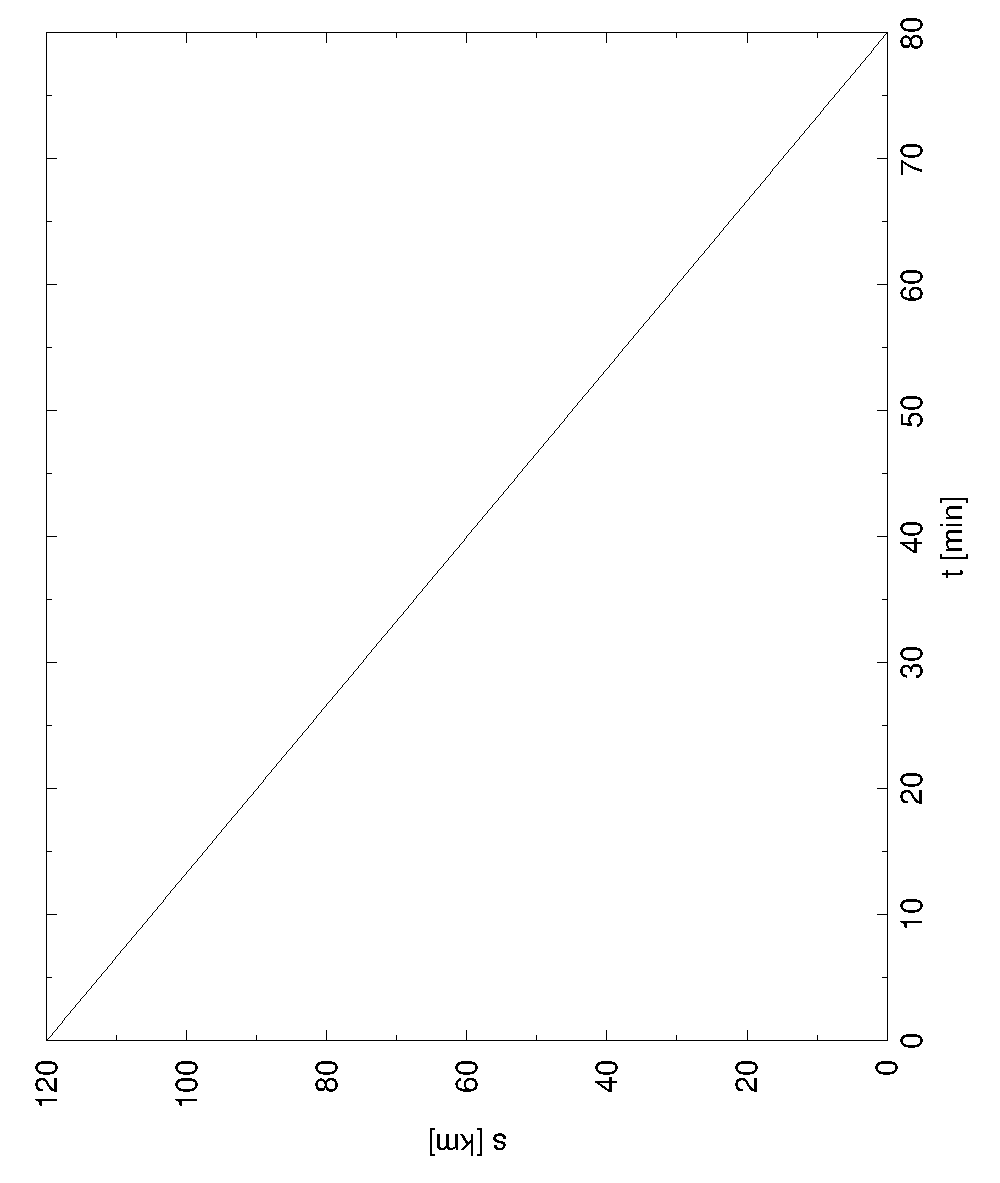
\includegraphics[angle=-90,width=0.8\linewidth]{pictures/zugkommt.eps}
\end{center}

\item $h_0=3\unit{m}$, $a=-0.35\ufrac{m}{h}$
  \begin{eqnarray*}
    h & = & at + h_0 \\
    h & = & \result{-0.35\ufrac{m}{h}\,t + 3\unit{m}}
  \end{eqnarray*}

\end{enumerate}}

\clearpage
\listoffigures
%\listoftables
%\newpage
%\nocite{*}
%\bibliographystyle{plain}
%\bibliography{preamble/literaturgoogle}
\end{document}